% A LaTeX template for MSc Thesis submissions to 
% Politecnico di Milano (PoliMi) - School of Industrial and Information Engineering
%
% S. Bonetti, A. Gruttadauria, G. Mescolini, A. Zingaro
% e-mail: template-tesi-ingind@polimi.it
%
% Last Revision: October 2021
%
% Copyright 2021 Politecnico di Milano, Italy. NC-BY

\documentclass{Configuration_Files/PoliMi3i_thesis}

%------------------------------------------------------------------------------
%	REQUIRED PACKAGES AND  CONFIGURATIONS
%------------------------------------------------------------------------------

% CONFIGURATIONS
\usepackage{parskip} % For paragraph layout
\usepackage{setspace} % For using single or double spacing
\usepackage{emptypage} % To insert empty pages
\usepackage{multicol} % To write in multiple columns (executive summary)
\setlength\columnsep{15pt} % Column separation in executive summary
\setlength\parindent{0pt} % Indentation
\raggedbottom  

% PACKAGES FOR TITLES
\usepackage{titlesec}
% \titlespacing{\section}{left spacing}{before spacing}{after spacing}
\titlespacing{\section}{0pt}{3.3ex}{2ex}
\titlespacing{\subsection}{0pt}{3.3ex}{1.65ex}
\titlespacing{\subsubsection}{0pt}{3.3ex}{1ex}
\usepackage{color}

% PACKAGES FOR LANGUAGE AND FONT
\usepackage[english]{babel} % The document is in English  
\usepackage[utf8]{inputenc} % UTF8 encoding
\usepackage[T1]{fontenc} % Font encoding
\usepackage[11pt]{moresize} % Big fonts

% PACKAGES FOR IMAGES
\usepackage{graphicx}
\usepackage{transparent} % Enables transparent images
\usepackage{eso-pic} % For the background picture on the title page
\usepackage{subfig} % Numbered and caption subfigures using \subfloat.
\usepackage{tikz} % A package for high-quality hand-made figures.
\usetikzlibrary{}
\graphicspath{{./Images/}} % Directory of the images
\usepackage{caption} % Coloured captions
\usepackage{xcolor} % Coloured captions
\usepackage{amsthm,thmtools,xcolor} % Coloured "Theorem"
\usepackage{float}

% STANDARD MATH PACKAGES
\usepackage{amsmath}
\usepackage{amsthm}
\usepackage{amssymb}
\usepackage{amsfonts}
\usepackage{bm}
\usepackage[overload]{empheq} % For braced-style systems of equations.
\usepackage{fix-cm} % To override original LaTeX restrictions on sizes

% PACKAGES FOR TABLES
\usepackage{tabularx}
\usepackage{longtable} % Tables that can span several pages
\usepackage{colortbl}

% PACKAGES FOR ALGORITHMS (PSEUDO-CODE)
\usepackage[ruled,vlined]{algorithm2e}

% PACKAGES FOR REFERENCES & BIBLIOGRAPHY
\usepackage[colorlinks=true,linkcolor=black,anchorcolor=black,citecolor=black,filecolor=black,menucolor=black,runcolor=black,urlcolor=black]{hyperref} % Adds clickable links at references
\usepackage{cleveref}
\usepackage[square, numbers, sort&compress]{natbib} % Square brackets, citing references with numbers, citations sorted by appearance in the text and compressed
\bibliographystyle{abbrvnat} % You may use a different style adapted to your field

% OTHER PACKAGES
\usepackage{pdfpages} % To include a pdf file
\usepackage{afterpage}
\usepackage{lipsum} % DUMMY PACKAGE
\usepackage{fancyhdr} % For the headers
\fancyhf{}

% Input of configuration file. Do not change config.tex file unless you really know what you are doing. 
% Set the geometric layout of the document
\usepackage{geometry}
\geometry{
  top=3cm,
  left = 2.0cm,
  right = 2.0cm,
  bottom=2cm,
  headheight= 2cm,
  headsep= 0cm,
}
\raggedbottom 

% Create color bluePoli (-> manuale grafica coordinata:  https://www.polimi.it/fileadmin/user_upload/il_Politecnico/grafica-coordinata/2015_05_11_46xy_manuale_grafica_coordinata.pdf)
\definecolor{bluePoli}{cmyk}{0.4,0.1,0,0.4}

% Custom theorem environments
\declaretheoremstyle[
  headfont=\color{bluePoli}\normalfont\bfseries,
  bodyfont=\color{black}\normalfont\itshape,
]{colored}

\captionsetup[figure]{labelfont={color=bluePoli}} % Set colour of the captions
\captionsetup[table]{labelfont={color=bluePoli}} % Set colour of the captions
\captionsetup[algorithm]{labelfont={color=bluePoli}} % Set colour of the captions

\theoremstyle{colored}
\newtheorem{theorem}{Theorem}[section]
\newtheorem{proposition}{Proposition}[section]

% Enhances the features of the standard "table" and "tabular" environments.
\newcommand\T{\rule{0pt}{2.6ex}}
\newcommand\B{\rule[-1.2ex]{0pt}{0pt}}

% Algorithm description
\newcounter{algsubstate}
\renewcommand{\thealgsubstate}{\alph{algsubstate}}
\newenvironment{algsubstates}{
    \setcounter{algsubstate}{0}%
    \renewcommand{\STATE}{%
    \stepcounter{algsubstate}%
    \Statex {\small\thealgsubstate:}\space}
    }{}
    
% Custom theorem environment
\newcolumntype{L}[1]{>{\raggedright\let\newline\\\arraybackslash\hspace{0pt}}m{#1}}
\newcolumntype{C}[1]{>{\centering\let\newline\\\arraybackslash\hspace{0pt}}m{#1}}
\newcolumntype{R}[1]{>{\raggedleft\let\newline\\\arraybackslash\hspace{0pt}}m{#1}}

% Custom itemize environment
\setlist[itemize,1]{label=$\bullet$}
\setlist[itemize,2]{label=$\circ$}
\setlist[itemize,3]{label=$-$}
\setlist{nosep}

% Set separation of columns 
\setlength{\columnsep}{30pt}

% Create command for background pic
\newcommand\BackgroundPic{% Adding background picture
	\put(230,358){
		\parbox[b][\paperheight]{\paperwidth}{%
			\vfill
			\centering
			\transparent{0.4}
			
\includegraphics[width=0.5\paperwidth]{raggiera_polimi.eps}%
			\vfill
}}}

% Set indentation
\setlength\parindent{0pt}

% Custom title commands
\titleformat{\section}
{\color{bluePoli}\normalfont\Large\bfseries}
{\color{bluePoli}\thesection.}{1em}{}
\titlespacing*{\section}
{0pt}{2ex}{1ex}

\titleformat{\subsection}
{\color{bluePoli}\normalfont\large\bfseries}
{\color{bluePoli}\thesubsection.}{1em}{}
\titlespacing*{\subsection}
{0pt}{2ex}{1ex}

% Custom headers and footers
\pagestyle{fancy}
\fancyhf{}
      
\fancyfoot{}
\fancyfoot[C]{\thepage} % page
\renewcommand{\headrulewidth}{0mm} % headrule width
\renewcommand{\footrulewidth}{0mm} % footrule width

\makeatletter
\patchcmd{\headrule}{\hrule}{\color{black}\hrule}{}{} % headrule
\patchcmd{\footrule}{\hrule}{\color{black}\hrule}{}{} % footrule
\makeatother

% -> Create the header
\chead[C]{
\centering
\begin{tcolorbox}[arc=0pt, boxrule=0pt, colback=bluePoli!60, width=\textwidth, colupper=white]
    \textbf{Executive summary} \hfill \textbf{\author}  
\end{tcolorbox}
}

%----------------------------------------------------------------------------
%	NEW COMMANDS DEFINED
%----------------------------------------------------------------------------

% EXAMPLES OF NEW COMMANDS
\newcommand{\bea}{\begin{eqnarray}} % Shortcut for equation arrays
\newcommand{\eea}{\end{eqnarray}}
\newcommand{\e}[1]{\times 10^{#1}}  % Powers of 10 notation

%----------------------------------------------------------------------------
%	ADD YOUR PACKAGES (be careful of package interaction)
%----------------------------------------------------------------------------

%----------------------------------------------------------------------------
%	ADD YOUR DEFINITIONS AND COMMANDS (be careful of existing commands)
%----------------------------------------------------------------------------
\theoremstyle{definition}
\newtheorem{definition}{Definition}[section]
\theoremstyle{observation}
\newtheorem{observation}{Observation}[section]

%----------------------------------------------------------------------------
%	BEGIN OF YOUR DOCUMENT
%----------------------------------------------------------------------------

\begin{document}

    \fancypagestyle{plain}{%
    \fancyhf{} % Clear all header and footer fields
    \fancyhead[RO,RE]{\thepage} %RO=right odd, RE=right even
    \renewcommand{\headrulewidth}{0pt}
    \renewcommand{\footrulewidth}{0pt}}
        
    %----------------------------------------------------------------------------
    %	TITLE PAGE
    %----------------------------------------------------------------------------

    \pagestyle{empty} % No page numbers
    \frontmatter % Use roman page numbering style (i, ii, iii, iv...) for the preamble pages

    \puttitle{
        title=Title, % Title of the thesis
        name=Name Surname, % Author Name and Surname
        course=Xxxxxxx Engineering - Ingegneria Xxxxxxx, % Study Programme (in Italian)
        ID  = 000000,  % Student ID number (numero di matricola)
        advisor= Prof. Name Surname, % Supervisor name
        coadvisor={Name Surname, Name Surname}, % Co-Supervisor name, remove this line if there is none
        academicyear={20XX-XX},  % Academic Year
    } % These info will be put into your Title page 

    %----------------------------------------------------------------------------
    %	PREAMBLE PAGES: ABSTRACT (inglese e italiano), EXECUTIVE SUMMARY
    %----------------------------------------------------------------------------
    \startpreamble
    \setcounter{page}{1} % Set page counter to 1

    \chapter{Abstract}\label{chapter:abstract}

    
% ABSTRACT IN ITALIAN
\chapter*{Abstract in lingua italiana}
I recenti progressi nella digitalizzazione dei processi industriali hanno portato a un aumento degli studi sul problema dell'imballaggio tridimensionale dei contenitori.
Il problema consiste nell'impacchettare un insieme di articoli nel numero minimo di contenitori senza alcuna sovrapposizione.
Quando si considerano istanze reali del problema, è necessaria l'aggiunta di nuovi vincoli pratici.
Studi precedenti in altri campi relativi al carico di container e pallet hanno dimostrato che la stabilità statica dei contenitori è un aspetto cruciale da considerare.
La maggior parte delle soluzioni in letteratura affronta il problema del supporto verticale implicitamente generando strati densi di articoli che vengono poi impilati per riempire un contenitore.
\\
In questa tesi, formuliamo un modello mixed-integer linear programming per il problema dell'imballaggio tridimensionale dei contenitori con una versione discretizzata del vincolo del supporto verticale.
Proponiamo poi un'euristica costruttiva che riempie i contenitori senza costruire esplicitamente soluzioni a strati o usare materiale di riempimento, come è solito in soluzioni dalla letteratura.
Inoltre, modifichiamo l'algoritmo bidimensionale Extreme Points per considerare il supporto verticale.
Introduciamo, poi, un algoritmo di beam-search che valuta diversi posizionamenti fatti dalla nostra euristica costruttiva e filtra le soluzioni duplicate.
Forniamo anche un set di istanze con articoli campionati da una popolazione di prodotti reali.
Infine, convalidiamo i risultati del nostro algoritmo usando diversi set di dati, sia dalla letteratura che da un caso di studio di pallettizzazione mista.
\\
\\
\textbf{Parole chiave:} imballaggio tridimensionale, supporto verticale, stabilità statica, pallettizzazione mista % Keywords (italian)

    %----------------------------------------------------------------------------
    %	LIST OF CONTENTS/FIGURES/TABLES/SYMBOLS
    %----------------------------------------------------------------------------

    % TABLE OF CONTENTS
    \thispagestyle{empty}
    \tableofcontents % Table of contents 
    \thispagestyle{empty}
    \cleardoublepage

    %-------------------------------------------------------------------------
    %	THESIS MAIN TEXT
    %-------------------------------------------------------------------------
    \addtocontents{toc}{\vspace{2em}} % Add a gap in the Contents, for aesthetics
    \mainmatter % Begin numeric (1,2,3...) page numbering

    % --------------------------------------------------------------------------
    % NUMBERED CHAPTERS % Regular chapters following
    % --------------------------------------------------------------------------
    \chapter*{Introduction}
    \label{chapter:introduction}%
    %More concise, add a bit of context on why they are importnat
The three-dimensional bin packing problem (3D-BPP) is part of the family of Cutting and Packing (C\&P) problems.
\cite{WASCHER20071109} identified a common structure for C\&P problems where, given two sets of small and large items, some or all small items need to be assigned to some or all large ones such that some geometric constraints are verified.
They also divided C\&Ps in several typologies based on the number of geometric dimensions (1D, 2D, 3D, nD), the kind of assignment to be made, the assortment of small items, the assortment of large items, and the shape of small items (regual or irregular).
The 3D-BPP involves packing, in three dimensions, a strongly heterogeneous assortment of small cuboid-shaped items of different size (boxes) into the minimum number of cuboid-shaped large ones (bins) without any overlap.
In the case of a 3D-BPP where the dimensions of the bins are also fixed, the problem is then defined as a Three-Dimensional Single Bin-Size Bin Packing Problem (3D-SBSBPP).
Items can only be placed with their edges parallel to the sides of the bin and, in some formulations, they can be rotated by $90$ degrees along their vertical axis.

In this thesis, we address a version of the 3D-SBSBPP stemming from a real case study of mixed-case palletization: the Three-Dimensional Bin Packing Problem with Vertical Support (3D-BPPVS).
Modeling real-world case studies with the 3D-SBSBPP requires additional constraints to be considered. We extend the standard formulation of the 3D-SBSBPP by ensuring that all items that are packed inside a bin will not fall, and we refer to this property as the vertical support.
Support constraints are usually defined based on the amount of area of an item that lies on top of other items, or by the number of corners of an item that rest on top of other items (\cite{GZARA20201062, paquay2016mixed, kurpel2020exact}).

The standard 3D-SBSBPP is strongly NP-hard since it is a generalization of the one-dimensional bin packing problem (\cite{martello2000three}).
Since our problem is a generalization of the 3D-SBSBPP, exact solution algorithms are only able to solve small instances of the problem; therefore, heuristic approaches need to be used to solve larger instances.
Heuristics designed to solve the 3D-SBSBPP do not address the concept of vertical support and allow solutions with unsupported items.
The concept of support has received most attention in Pallet Loading Problems and Container Loading Problems (\cite{Calzavara2021, kurpel2020exact}).
These problems involve an assortment of weakly heterogeneous items and were classified by \cite{WASCHER20071109} as Cutting Stock problems.
Since items can be easily grouped together, the concept of support is addressed explicitly by building layers or walls of items with high density. This allows to reduce the problem to a one-dimensional packing problem (\cite{BORTFELDT20131}).
In mixed-case palletization scenarios, layer-based solutions represent the majority of work in the literature. They usually work by stacking layers ordered by density until the density of the last generated layers falls below a certain threshold.
Once no more layers can be generated, simpler techniques are employed to pack the remaining items (\cite{elhedhli2019three}), or the use of filler boxes is employed to increase the layer's density (\cite{Calzavara2021}).

In this thesis we
\begin{itemize}
    \item formulate a mixed-integer linear programming model for the 3D-BPPVS with a discretized version of the support constraint,
    \item develop a constructive heuristic that fills bins while guaranteeing vertical support, without explicitly building layered solutions or using filler boxes,
    \item introduce a beam search heuristic that expands the constructive heuristic's solution space by exploring different orders of item palletization,
    \item validate the proposed heuristic against our model and against the most relevant heuristics from the 3D-SBSBPP literature,
    \item generate and share a data set based on real-world instances that we use to benchmark our heuristic.
\end{itemize}

\section{Case study}
\label{sec:intro:case_study}%
The work of this thesis stems from the case study of a logistics company in northern Italy.
The company manages large warehouses where automated lines bring boxes to different packing stations, and then they are loaded onto pallets of standard size.
Each box is then loaded manually by an operator, and as soon as the height of the pallet reaches a certain threshold, the packing station lowers it and wraps it with an elastic material that guarantees its stability.
This wrapping improves the stability of the pallet while boxes are still being loaded on the top. To avoid uneven surfaces during the wrapping phase, pallets should not have empty spaces inside.
Since the company is dealing directly with customers' orders, boxes have very different sizes and are usually packed in smaller quantities. This implies that layer-based pallet loading solutions are impractical in these cases, since it is usually not possible to build full layers of boxes of the same height.
The company is interested in building pallets that do not have empty spaces inside, and they measure this property with a metric called cage ratio.
The cage ratio measures the ratio between the volume of items packed inside a bin and the volume of the cuboid with the same base as the bin and height equal to the highest item inside the bin.
This measurement is a good indicator of unused space under the highest item in the bin.
To increase the efficiency of the wrapping and to allow for the stacking of pallets, solutions with a high cage ratio are required.
The cage ratio of commercial solutions currently implemented by the company is around $60\%$, and a target cage ratio for our case study was set at $70\%$.

\newpage
\section{Overview}
\label{sec:intro:overview}%
In \cref{chapter:literature} we review the relevant literature on the three-dimensional bin packing problems and the cutting and packing problems dealing with vertical support.
In \cref{chapter:problem} we give a formal definition of the problem and formulate a mixed-integer linear programming model that we will use to validate the proposed solution algorithm.
Since the model can not be used to solve real-world instances, in \cref{chapter:heuristics} we propose a heuristic algorithm that is able to solve larger problem instances.
In \cref{chapther:experiments} we present our computational experiments. We compare our heuristic algorithm against relevant heuristics from the literature, solutions from our MILP model, and against solutions from our real-world case study. We also describe the process that we used to generate new instances.
Finally, in \cref{chapther:conclusions} we provide final remarks and list possible further developments of this research.

    \chapter{Literature review}
    \label{chapter:literature}%
    %Overview of section
In this section we review the relevant literature to our problem. 
In \cref{sec:literature:2dbpp} we do a brief review of the most relevant two-dimensional bin packing placement heuristics in the context of this thesis.
In \cref{sec:literature:3dbpp} we review the literature on the 3D-BPP with a focus on the heuristics used to solve the single bin-size bin packing problem.
Finally, in \cref{sec:literature:support} we do a brief review of the literature on practical constraints in cutting and packing problems with a focus on the vertical support constraint.

\section{Two-Dimensional Bin Packing Problem}
\label{sec:literature:2dbpp}%
In the two-dimensional bin packing problem two major tasks constitute the area of study which is relevant to constructive heuristic. 
The first task is to identify the smallest set of points where a placement can be made.
The second task consists in evaluating which point to select for a placement, the main strategies are divided in first-fit and best-fit approaches.
In first-fit approaches the first valid positions are selected while in best-fit approaches positions are selected based on a metric.
The most common classical algorithm to select placements inside a two-dimensional bin given a set of points is the bottom-most left-most algorithm introduced in \cite{Baker1980}. 
It packs items in the lowest possible position closest to the bottom-left corner of the free area. 
This algorithm serves as the base of a lot of heuristics that address the two-dimensional bin packing problem (2D-BPP).
In \cite{burke2004new} a best-fit algorithm is introduced where placements of items that fit the lowest available area are made first.
In \cite{lodi1999heuristic} a maximum touching perimeter approach is used instead.

Considering the identification of possible packing positions, in \cite{Martello1998} a branch-and-bound algorithm was proposed to solve the two-dimensional orthogonal packing problem (2D-OPP).
The selection of the positions is done with a left-most downwards strategy where items are placed in a way such that their left and bottom edges touch either other items or the bin.
The algorithm is based on a tree-search that packs items in every possible position.
It was also embedded in an enumeration algorithm to solve the 2D-BPP, and a set of 10 classical instances to benchmark heuristics against were presented.
In \cite{martello2003exact} a branch-and-bound algorithm for the two-dimensional strip packing problem (2D-SPP) was proposed, based on the idea of staircase placements introduced in \cite{scheithauer1995equivalence}.
In staircase placements a boundary is identified which separates the already packed items from the area that is still free.
This boundary, called the envelope, is composed of segments that touch either the side of an item or the bin.
In the formed staircase-like shape, the corner points are then points where the envelope changes from horizontal to vertical.
A similar approach was then used in \cite{crainic2008extreme} where an extension to the staircase approach was introduced with the concept of extreme points.
In the proposed method, each packed item introduces a fixed number of extreme points which are the projection of his corner points along the orthogonal axis onto the sides of either the bin or its closest packed neighbour.
This allowed to identify niches that were previously discarded by the staircase method.
Both the extreme point and corner point strategies were adapted to the three-dimensional bin packing case as seen in \cref{sec:literature:3dbpp}.

For a recent review of the literature related to the 2D-BPP we refer the reader to \cite{IORI2021399} which conducted a survey of two dimensional packing problem with formulations of the problem, heuristic and exact methods, relaxations and open problems.

\section{Three-Dimensional Single Bin-Size Bin Packing Problem}
\label{sec:literature:3dbpp}%

An exact approach to the 3D-SBSBPP was proposed in \cite{martello2000three} through a two-level branch-and-bound search and the use of a staircase placement method derived from the 2D-BPP field.
The algorithm was initially limited to robot packable solutions, and was then extended to the general problem in \cite{martello2007exact}.
\cite{faroe2003guided} proposed a Guided Local Search for both the 2D-SBSBPP and 3D-SBSBPP.
Starting from a upper bound on the number of bins calulated through a greedy heuristic it iteratively improved the solutions by searching for new feasible solutions thanks to the proposed GLS method.
The process terminated when either a computed lower bound was reached or a certain time limit had expired.
In \cite{lodi2002heuristic} a tabu search procedure that addresses the two-dimensional and three-dimensional bin packing case was proposed.
The search was based on two steps, starting with one item per bin a certain number of bins were merged together. 
Two constructive heuristics were then used to create layers in each bin.
Between each step a 1D-BPP was solved to stack the generated layers into bins.
\cite{Lodi2004} later provided code for a unified tabu search addressing the multi-dimensional bin packing problem.
A two-level tabu search for the multi-dimensional bin packing problem was provided in \cite{crainic2009ts2pack}.
The algorithm started from a greedy feasible solution based on the extreme point heuristic introduced in \cite{crainic2008extreme}.
In the first step of the algorithm they built a neighbourhood by swapping or moving items between bins while relaxing the bin constraints.
In the second step they searched for feasible solutions by changing the relative positions of items inside of the bin. %TODO: maybe fekete here?
In \cite{fekete2004combinatorial} a new model for bin packing problem based on interval graphs was introduced. 
A packing was represented as an interval graph of the overlaps of items along each axis.
A GRASP-based algorithm for the 3D-SBSBPP and 2D-SBSBPP was proposed by \cite{parreno2010hybrid}, the algorithm uses a maximal-space heuristich designed for container loading problems during its constructive phase.
Serveral moves were then designed and combined in an improvement phase with a variable neighbourhood descent approach.
In \cite{WU2010347} a genetic algorithm was presented which varied the relative positions of items in a mixed-integer linear programming model. The chromosomes represented the order of items to be packed and their orientation.
\cite{hifi2014hybrid} proposed a hybrid greedy heuristic which solves the 3D-SBSBPP in two phases; 
a selection phase where a subset of items to pack as a solution to a knapsack problem and a positioning phase the fixes the position of each item inside the bins.
In both phases an integer linear programming model is employed. An additional optimization phase can also introduced at the cost of computational times.
\cite{gonccalves2013biased} presented a biased random-key genetic algorithm for the 3D-SBSBPP (BRKGA).
The chromosomes reppresented the encoding for the sequence of packing of each item.
The packing was done with an underlying heuristic that uses the same maximal-space rapresentation as \citet{parreno2010hybrid}.
\cite{zudio2018brkga} later proposed a variable neighbourhood descent variation of BRKGA which improved the evolving process of BRKGA by finding high quality individuals in earlier generations.

%Space Defrag in BPP {Zhu and Lim (2012)}
%A column-generation approach was proposed in \cite{ZHU2012452}
%The work was then used in \cite{ZHU2012408} in combination with a greedy-lookahead tree search to solve the single container loading problem.

%TODO: Bounds?
\section{Vertical Support}
\label{sec:literature:support}%
Vertical support (or static stability) received most of its contributions from the fields of Pallet Loading Problems (PLP) and Cargo Loading Problems (CLP).
In recent years there has been lots of pubblications addressing various practical constraints dictated by the industry needs.
In this section we focus on pubblications related to these two problems that dealt with the concept of vertical support.

As noted in \cite{BORTFELDT20131}, static stability is one of the most important constraints in Cargo Loading Problems but it is usually implicitly enforced as a consequence of load compactness or explicitly guaranteed by using filler material as a postprocessing step.
A MIP formulation was proposed in \cite{paquay2016mixed} with the inclusion of various practical constraints like vertical support through vertex support, containers of different size and shape, weight distribution, item rotations and load bearing.
Since the proposed model was complex, only small instances were solved to optimality in a reasonable time frame. The work was extended in \cite{paquay2007} where three meta-heuristics were provided to reduce the solve time.
In \cite{GALRAORAMOS2016565} the single container CLP is solved with static mechanical stability by combining a multi-polulation random key genetic algorithm (BRKGA) with a constructive heuristich which determins a two-dimensional box placement strategy.
The pubblication also proposed a procedure to fill maximal-spaces based on mechanichal equilibrium conditions applyed to rigidbodies.
In \cite{kurpel2020exact} several new formulations of CLP are presented with various extensions for practical constraints such as box orientations, stability (including vertical support) and the separation of boxes.
Vertical Support is formulated by a discretization of space along each axis and with the help of an overlap matrix to encode the ammount of area support each item can give to the others.
The work also presents heuristic approaches and upper and lower bound techniques.
In \cite{Alonso2020} a multi container loading problem is solved by using a GRASP meta-heuristich where pallets are built from a set of layers and then positioned inside a container. 
Practical constraints are considered like weight limits, weight distribution, dynamic stability, delivery dates. The constraint of static stability is implicitly ensured by building dense layers.
In \cite{GAJDA2022102559} a constructive randomized heuristic for solving the CLP is proposed with constraints including vertical support ensured by area support, customer priorities, load balancing, stacking constraints, and positioning constraints.
In the proposed constructive heuristic a subset of extreme points are evaluated starting from two corners of the cargo to ensure a better weight distribution.

Considering Pallet Loading Problems, in \cite{elhedhli2019three} a column-generation framework and a branch-and-price solution to the mixed-case pallet loading problem was proposed with a two-dimensional layer generation problem as the pricing subproblem.
The subproblem was then solved with exact methods and heuristically with additions including item groupings, item replacement the reoganization of layers and spacing.
A new instance generator for instances that better reppresent industry instances was provided. The paper didn't directly address vertical support although the layering approach used implicitly favored solutions with support.
The work was later extended by \cite{GZARA20201062} to explicitly address practical constraints such as vertical support, load bearing, pallet weight limits and planogram sequencing.
A second-order cone programming formulation was provided as a solution to a spacing problem between layers of a pallet and further extensions to the previously introduced instance generator were made.
In \cite{Calzavara2021} a mathematical formulation for a layer and a pallet generation problem are defined together with heuristics and metaheuristics algorithms designed to solve the PLP with constraints on item groupings, layering, and visibility of items.
The work is based on previous papers on PLP by the same authors \cite{Iori2020a, Iori2020b, Iori2021} that proposed a raective GRASP metaheuristic to solve the general problem.
Stability of the solutions is implicitly ensured with layering and the use of filler boxes to increase the density of problematic layers.

    \chapter{Problem description and mathematical formulation}
    \label{chapter:problem}%
    \section{3D Bin Packing Problem}

\section{Support} %TODO: Here or in introduction?

\section{MILP Formulation}
\label{sec:milp}%
\subsection*{Conceptual model}
A conceptual model of the problem we are trying to solve would be:

%TODO: Cage Ratio?
\begin{align*}
    \textbf{minimize} \hspace{.5cm}   & \text{unused volume in used bins} \\
    \textbf{subject to} \hspace{.5cm} & \text{all items assigned to one and only one bin} \\
                                      & \text{all items within the bin dimensions} \\
                                      & \text{no overlaps between items in the same bin} \\
                                      & \text{all items with support} \\
\end{align*}

We can now provide the formal definition of the 3DBPP by formulating a mixed integer linear programming problem model.

\subsection*{Formal model}
\label{ssec:formal_model}
We'll now introduce a MILP model for the standard 3DBPP problem definition and then we'll expand it to address the stability constraint afterwards.

We start by defining the known sets and parameters of the problem.
\paragraph*{Sets}
\begin{align*}
    I = \{1,\dots, n \}: \hspace{.5cm}& \text{set of items} \\
    B = \{1,\dots, m \}: \hspace{.5cm}& \text{set of bins} 
\end{align*}
\paragraph*{Parameters}
\begin{align}
          W \times D \times H  \hspace{.5cm}& \text{width $\times$ depth $\times$ height of a bin} \notag \\
                            V  \hspace{.5cm}& \text{bin volume} \notag \\
    w_i \times d_i \times h_i  \hspace{.5cm}& \text{width $\times$ depth $\times$ height of item $i$} & \forall i \in I \label{par:item_dim}
\end{align}

\paragraph*{Variables} We can now introduce the following sets of integer variables
\begin{align}
              (x_i,y_i,z_i) \hspace{.5cm}& \text{bottom front left corner of an item} & \forall i \in I \label{var:item_pos} \\
    (x^\prime_i,y^\prime_i) \hspace{.5cm}& \text{back right corner of an item} & \forall i \in I \label{var:item_back_pos} \\
                        r_i \hspace{.5cm}& \begin{cases}
                                            1, \text{if item $i$ is rotated 90° over its z-axis} \\ 
                                            0, \text{otherwise}
                                        \end{cases} & \forall i \in I \label{var:item_rot} \\
                    u_{ib} \hspace{.5cm}& \begin{cases}
                                            1, \text{if item $i$ is placed in bin $b$} \\ 
                                            0, \text{otherwise}
                                        \end{cases} & \forall i \in I, \forall b \in B \notag \\
                    x^p_{ij} \hspace{.5cm}& \begin{cases}
                                            1, \text{if $x_i \le x^\prime_j$} \\ 
                                            0, \text{otherwise}
                                        \end{cases} & \forall i,j \in I \notag \\
                    y^p_{ij} \hspace{.5cm}& \begin{cases}
                                            1, \text{if $y_i \le y^\prime_j$} \\ 
                                            0, \text{otherwise}
                                        \end{cases} & \forall i,j \in I \notag \\
                    z^p_{ij} \hspace{.5cm}& \begin{cases}
                                            1, \text{if $z_i \le z_j + h_j$} \\ 
                                            0, \text{otherwise}
                                        \end{cases} & \forall i,j \in I \notag \\
            z_b^\text{max} \hspace{.5cm}& \text{maximum height of bin $b$} & \forall b \in B \notag
\end{align}

Given a coordinate system, each item $i$ can be represented univocally in 3D space by \cref{par:item_dim,var:item_pos,var:item_back_pos,var:item_rot} as seen in figure \ref{fig:coordinate_system}
\begin{figure}
    \scalebox{0.65}{%
    

\tikzset{every picture/.style={line width=0.75pt}} %set default line width to 0.75pt        

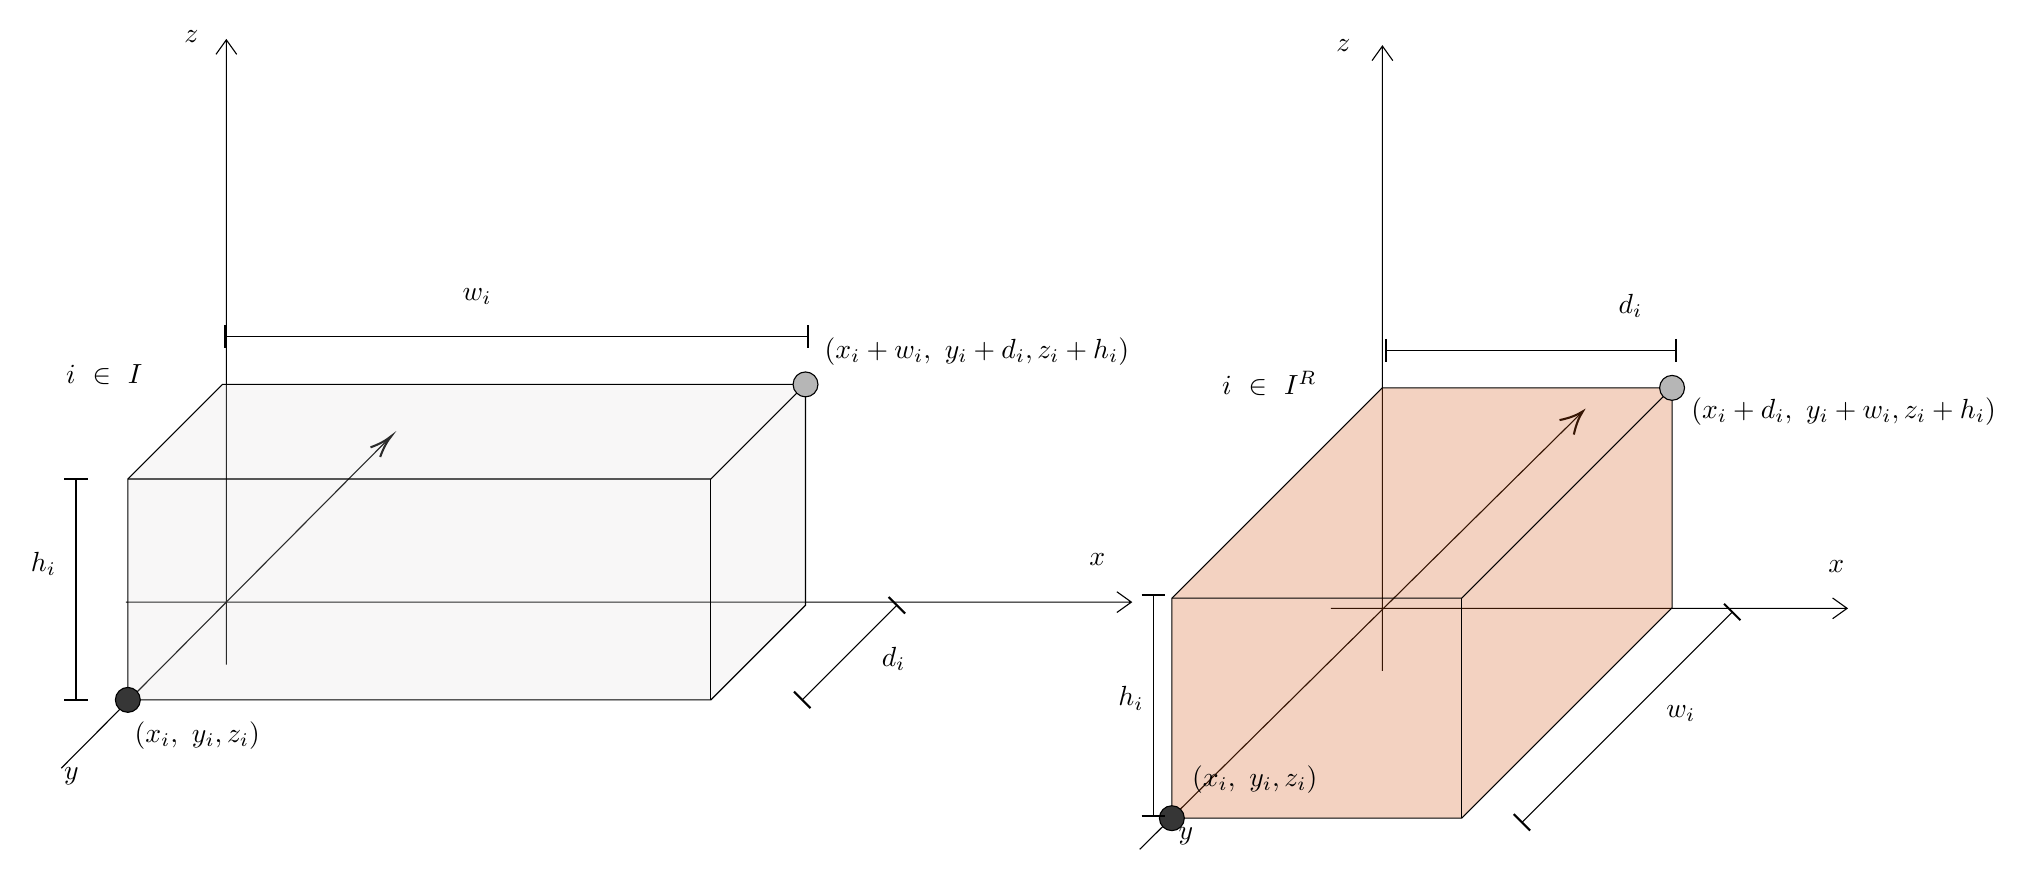
\begin{tikzpicture}[x=0.75pt,y=0.75pt,yscale=-1,xscale=1]
%uncomment if require: \path (0,479); %set diagram left start at 0, and has height of 479

%Shape: Axis 2D [id:dp17090047473688563] 
\draw  (122,295.9) -- (606.5,295.9)(170.45,25) -- (170.45,326) (599.5,290.9) -- (606.5,295.9) -- (599.5,300.9) (165.45,32) -- (170.45,25) -- (175.45,32)  ;
%Straight Lines [id:da9671294084497354] 
\draw    (248.54,217.32) -- (90.95,375.9) ;
\draw [shift={(249.95,215.9)}, rotate = 134.82] [color={rgb, 255:red, 0; green, 0; blue, 0 }  ][line width=0.75]    (10.93,-3.29) .. controls (6.95,-1.4) and (3.31,-0.3) .. (0,0) .. controls (3.31,0.3) and (6.95,1.4) .. (10.93,3.29)   ;
%Shape: Cube [id:dp18105788479145446] 
\draw  [fill={rgb, 255:red, 218; green, 217; blue, 217 }  ,fill opacity=0.2 ] (123,236.6) -- (168.6,191) -- (449.5,191) -- (449.5,297.4) -- (403.9,343) -- (123,343) -- cycle ; \draw   (449.5,191) -- (403.9,236.6) -- (123,236.6) ; \draw   (403.9,236.6) -- (403.9,343) ;
%Flowchart: Connector [id:dp700077731080137] 
\draw  [fill={rgb, 255:red, 54; green, 54; blue, 54 }  ,fill opacity=1 ] (117,343) .. controls (117,339.69) and (119.69,337) .. (123,337) .. controls (126.31,337) and (129,339.69) .. (129,343) .. controls (129,346.31) and (126.31,349) .. (123,349) .. controls (119.69,349) and (117,346.31) .. (117,343) -- cycle ;
%Flowchart: Connector [id:dp7959957780151166] 
\draw  [fill={rgb, 255:red, 182; green, 182; blue, 182 }  ,fill opacity=1 ] (443.5,191) .. controls (443.5,187.69) and (446.19,185) .. (449.5,185) .. controls (452.81,185) and (455.5,187.69) .. (455.5,191) .. controls (455.5,194.31) and (452.81,197) .. (449.5,197) .. controls (446.19,197) and (443.5,194.31) .. (443.5,191) -- cycle ;
%Straight Lines [id:da2736427434795695] 
\draw    (169.6,168) -- (450.5,168) ;
\draw [shift={(450.5,168)}, rotate = 180] [color={rgb, 255:red, 0; green, 0; blue, 0 }  ][line width=0.75]    (0,5.59) -- (0,-5.59)   ;
\draw [shift={(169.6,168)}, rotate = 180] [color={rgb, 255:red, 0; green, 0; blue, 0 }  ][line width=0.75]    (0,5.59) -- (0,-5.59)   ;
%Straight Lines [id:da5491305384137963] 
\draw    (447.9,343) -- (493.5,297.4) ;
\draw [shift={(493.5,297.4)}, rotate = 135] [color={rgb, 255:red, 0; green, 0; blue, 0 }  ][line width=0.75]    (0,5.59) -- (0,-5.59)   ;
\draw [shift={(447.9,343)}, rotate = 135] [color={rgb, 255:red, 0; green, 0; blue, 0 }  ][line width=0.75]    (0,5.59) -- (0,-5.59)   ;
%Straight Lines [id:da2096690092171385] 
\draw    (98,343) -- (98,236.6) ;
\draw [shift={(98,236.6)}, rotate = 90] [color={rgb, 255:red, 0; green, 0; blue, 0 }  ][line width=0.75]    (0,5.59) -- (0,-5.59)   ;
\draw [shift={(98,343)}, rotate = 90] [color={rgb, 255:red, 0; green, 0; blue, 0 }  ][line width=0.75]    (0,5.59) -- (0,-5.59)   ;
%Shape: Axis 2D [id:dp7776925959360946] 
\draw  (702.58,298.9) -- (951.33,298.9)(727.45,28) -- (727.45,329) (944.33,293.9) -- (951.33,298.9) -- (944.33,303.9) (722.45,35) -- (727.45,28) -- (732.45,35)  ;
%Straight Lines [id:da8573442295183169] 
\draw    (822.58,205.41) -- (610.5,415) ;
\draw [shift={(824,204)}, rotate = 135.34] [color={rgb, 255:red, 0; green, 0; blue, 0 }  ][line width=0.75]    (10.93,-4.9) .. controls (6.95,-2.3) and (3.31,-0.67) .. (0,0) .. controls (3.31,0.67) and (6.95,2.3) .. (10.93,4.9)   ;
%Shape: Cube [id:dp7879935806557912] 
\draw  [color={rgb, 255:red, 0; green, 0; blue, 0 }  ,draw opacity=1 ][fill={rgb, 255:red, 209; green, 82; blue, 15 }  ,fill opacity=0.26 ] (626,294) -- (727.33,192.67) -- (867,192.67) -- (867,298.67) -- (765.67,400) -- (626,400) -- cycle ; \draw  [color={rgb, 255:red, 0; green, 0; blue, 0 }  ,draw opacity=1 ] (867,192.67) -- (765.67,294) -- (626,294) ; \draw  [color={rgb, 255:red, 0; green, 0; blue, 0 }  ,draw opacity=1 ] (765.67,294) -- (765.67,400) ;
%Flowchart: Connector [id:dp1932349089965345] 
\draw  [fill={rgb, 255:red, 54; green, 54; blue, 54 }  ,fill opacity=1 ] (620,400) .. controls (620,396.69) and (622.69,394) .. (626,394) .. controls (629.31,394) and (632,396.69) .. (632,400) .. controls (632,403.31) and (629.31,406) .. (626,406) .. controls (622.69,406) and (620,403.31) .. (620,400) -- cycle ;
%Flowchart: Connector [id:dp6515973139480861] 
\draw  [fill={rgb, 255:red, 182; green, 182; blue, 182 }  ,fill opacity=1 ] (861,192.67) .. controls (861,189.36) and (863.69,186.67) .. (867,186.67) .. controls (870.31,186.67) and (873,189.36) .. (873,192.67) .. controls (873,195.99) and (870.31,198.67) .. (867,198.67) .. controls (863.69,198.67) and (861,195.99) .. (861,192.67) -- cycle ;
%Straight Lines [id:da6236125294574628] 
\draw    (729.33,174.67) -- (869,174.67) ;
\draw [shift={(869,174.67)}, rotate = 180] [color={rgb, 255:red, 0; green, 0; blue, 0 }  ][line width=0.75]    (0,5.59) -- (0,-5.59)   ;
\draw [shift={(729.33,174.67)}, rotate = 180] [color={rgb, 255:red, 0; green, 0; blue, 0 }  ][line width=0.75]    (0,5.59) -- (0,-5.59)   ;
%Straight Lines [id:da29019630748971836] 
\draw    (794.67,402) -- (896,300.67) ;
\draw [shift={(896,300.67)}, rotate = 135] [color={rgb, 255:red, 0; green, 0; blue, 0 }  ][line width=0.75]    (0,5.59) -- (0,-5.59)   ;
\draw [shift={(794.67,402)}, rotate = 135] [color={rgb, 255:red, 0; green, 0; blue, 0 }  ][line width=0.75]    (0,5.59) -- (0,-5.59)   ;
%Straight Lines [id:da5655913131564809] 
\draw    (617,399) -- (617,292.6) ;
\draw [shift={(617,292.6)}, rotate = 90] [color={rgb, 255:red, 0; green, 0; blue, 0 }  ][line width=0.75]    (0,5.59) -- (0,-5.59)   ;
\draw [shift={(617,399)}, rotate = 90] [color={rgb, 255:red, 0; green, 0; blue, 0 }  ][line width=0.75]    (0,5.59) -- (0,-5.59)   ;

% Text Node
\draw (125,352.4) node [anchor=north west][inner sep=0.75pt]    {$( x_{i} ,\ y_{i} ,z_{i})$};
% Text Node
\draw (457.45,167.3) node [anchor=north west][inner sep=0.75pt]    {$\left( x_{i} + w_{i} ,\ y_{i} + d_{i} ,z_{i} +h_{i}\right)$};
% Text Node
\draw (92,180.4) node [anchor=north west][inner sep=0.75pt]    {$i \ \in\ I$};
% Text Node
\draw (283,143.4) node [anchor=north west][inner sep=0.75pt]    {$w_{i}$};
% Text Node
\draw (485,316.4) node [anchor=north west][inner sep=0.75pt]    {$d_{i}$};
% Text Node
\draw (75,270.4) node [anchor=north west][inner sep=0.75pt]    {$h_{i}$};
% Text Node
\draw (634.45,373.3) node [anchor=north west][inner sep=0.75pt]    {$( x_{i} ,\ y_{i} ,z_{i})$};
% Text Node
\draw (875,196.07) node [anchor=north west][inner sep=0.75pt]    {$\left( x_{i} + d_{i} ,\ y_{i} + w_{i} ,z_{i} +h_{i}\right)$};
% Text Node
\draw (649,183.4) node [anchor=north west][inner sep=0.75pt]    {$i \ \in\ I^R$};
% Text Node
\draw (840,146.4) node [anchor=north west][inner sep=0.75pt]    {$d_{i}$};
% Text Node
\draw (863,344.4) node [anchor=north west][inner sep=0.75pt]    {$w_{i}$};
% Text Node
\draw (599,335.4) node [anchor=north west][inner sep=0.75pt]    {$h_{i}$};
% Text Node
\draw (149,19.4) node [anchor=north west][inner sep=0.75pt]    {$z$};
% Text Node
\draw (704,23.4) node [anchor=north west][inner sep=0.75pt]    {$z$};
% Text Node
\draw (941,274.4) node [anchor=north west][inner sep=0.75pt]    {$x$};
% Text Node
\draw (585,271.4) node [anchor=north west][inner sep=0.75pt]    {$x$};
% Text Node
\draw (91,374.4) node [anchor=north west][inner sep=0.75pt]    {$y$};
% Text Node
\draw (628,403.4) node [anchor=north west][inner sep=0.75pt]    {$y$};


\end{tikzpicture}

    }
    \caption{Coordinate system representation for a generic item $i$ given its rotation $r_i$ 
    \label{fig:coordinate_system}}
\end{figure}

\subsection*{Static stability constraints}

We now extend the model introduced in \cref{ssec:formal_model} to introduce constraints addressing static stability.

\paragraph*{Additional Parameters}
\begin{align*}
    \alpha_s  :\hspace{.5cm}& \text{support area threshold} \\
    \beta_s  :\hspace{.5cm}& \text{support height tolerance} 
\end{align*}

    \chapter{Solution algorithms}
    \label{chapter:heuristics}%
    In this chapter we present our heuristic algorithm to solve the 3D-BPPVS. 
Since the 3D-BPP is NP-Hard, an exhaustive search for a solution is not practical, therefore a heuristic search is conducted by combining the beam search algorithm described in \cref{sec:beamsearch} with the constructive heuristic described in \cref{sec:support_planes}.
In section \ref{sec:problem_state} we define the preliminary concepts that will be used in the algorithm: states, insertions and solution's feasibility.

%TODO: Explain a bit why support planes instead of layers
\section{States}
\label{sec:problem_state}%
States are partial solutions of the 3D-BPPVS. Since our heuristic is based on a constructive method, starting from a state representing an empty solution we will iteratively build new states that gradually change to become a complete solution of the problem.
Being a partial solution, a state $s$ can be represented using the set of all variables present in the MILP model (\ref{sec:milp}), where some values have been fixed. 
Without loss of generality some of the notation defined in \cref{chapter:problem} is modified to include an index $s$ of the state we are considering.
We move closer to a complete solution of the problem by packing more items and opening new bins, i.e., by fixing more variables.

In order to simplify the algorithm's description, we introduce a few new definitions.
\begin{definition}[Open bin]
    A bin $b \in B$ is open in state $s$ \textbf{iff}
    \begin{equation*}
        v^{s}_{b} = 1
    \end{equation*}
\end{definition}

\begin{definition}[Set of open bins]
    Let $s$ be a state, we define $B^s$ as the set of bins that are open in $s$.
    \begin{equation*}
        B^s = \{ b \in B \mid v^{s}_{b} = 1 \}
    \end{equation*}
\end{definition}

\begin{definition}[Unpacked item]
    An item $i \in I$ is unpacked in state $s$ \textbf{iff}
    \begin{equation*}
        \sum_{b \in B} u^{s}_{ib} = 0
    \end{equation*}
    ,i.e., it has yet to be assigned to an open bin.
\end{definition}

\begin{definition}[Set of unpacked items]
    Let $s$ be a state, we define $U^s$ as the set of unpacked items in $s$.
    \begin{equation*}
        U^s = \{ i \in I \mid \sum_{b \in B} u^{s}_{ib} = 0 \}
    \end{equation*}
\end{definition}

\begin{definition}[Set of packed items]
    Let $s$ be a state and let $b \in B^s$, we define $J^s_b$ as the set of items that are packed inside $b$.
    \begin{equation*}
        J^s_b = \{ i \in I \mid u^{s}_{ib} = 1 \}
    \end{equation*}
\end{definition}

Due to these new definitions, we can define a function that determines if a state is a final state.
\begin{definition}
    \label{def:state_final}
    A state $s$ is final if there are no more items to pack.
    \begin{equation}
        \label{algo:state_final}%
        IsFinal(s) = \left\{\begin{aligned}
            1,\hspace{0.5cm}& U^s = \emptyset \\
            0,\hspace{0.5cm}& \text{otherwise}
        \end{aligned}
        \right.
    \end{equation}
\end{definition}

We can also define the empty state, which will be used as a starting point for our algorithm.
\begin{definition}[Empty state] \label{def:empty_state}
    A state $s$ is empty if it contains a single open bin without any item packed inside.
    \begin{equation*}
        U^s = I \wedge |B^s| = 1
    \end{equation*}
    By problem definition, the first expression implies that $J^s_b = \varnothing$ $\forall b \in B^s$.
\end{definition}

Given a state $s$, for each item $i \in I$ packed in $b \in B^s$ ($i \in J^s_b$), we let $(x^s_i, y^s_i, z^s_i)$ be the coordinates of its bottom front left corner. In order to simplify the algorithm representation, rotations are handled implicitly by swapping the dimensions $w_i$ and $d_i$ of item $i \in I$ when needed. An item can have different rotations if packed in different states, therefore we use its horizontal dimensions as variables and refer to them with $w^s_i$ and $d^s_i$.

\subsection{Axis-Aligned Bounding Box Tree}
\label{sec:problem_state:aabbtree}%

To determine the feasibility of a given state, one needs to check if no placed items overlap.
Since every item is a cuboid and our problem formulation only allows for $90\deg$ rotations over the z-axis, each item is contained inside a bounding box, which is axis-aligned.
An adequate structure to compute overlaps is then an Axis-Aligned Bounding Box Tree (AABB Tree) \citep{bergen1997efficient}.
The concept of using AABB Trees in three-dimensional bin packing heuristics was already a studied in the literature (e.g., \cite{ALLEN2011219}).
A conceptual image of a two-dimensional AABB Tree which contains three elements can be seen in \cref{fig:aabb_tree}.

\begin{figure}
    \label{fig:aabb_tree}%
    

\tikzset{every picture/.style={line width=0.75pt}} %set default line width to 0.75pt        

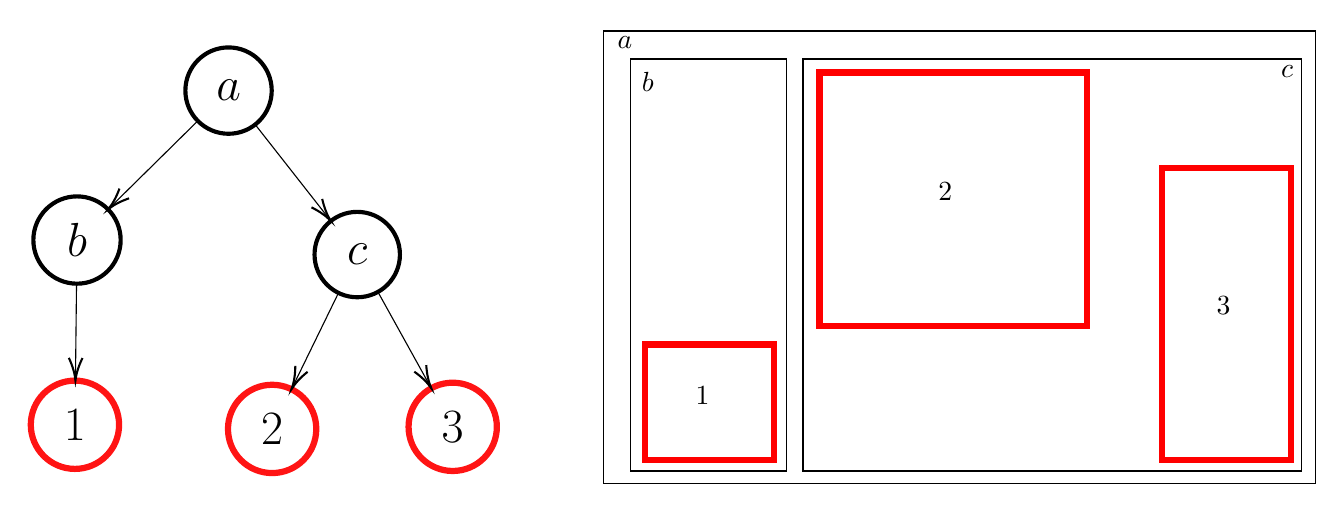
\begin{tikzpicture}[x=0.75pt,y=0.75pt,yscale=-1,xscale=1]
%uncomment if require: \path (0,269); %set diagram left start at 0, and has height of 269

%Shape: Rectangle [id:dp45712367712220003] 
\draw   (314,16.5) -- (657,16.5) -- (657,234.5) -- (314,234.5) -- cycle ;
%Shape: Rectangle [id:dp4249683313230568] 
\draw   (327,30) -- (402,30) -- (402,228.5) -- (327,228.5) -- cycle ;
%Shape: Rectangle [id:dp35105668268883494] 
\draw   (410,30) -- (650,30) -- (650,228.5) -- (410,228.5) -- cycle ;
%Shape: Rectangle [id:dp8308248735679132] 
\draw  [color={rgb, 255:red, 255; green, 0; blue, 0 }  ,draw opacity=1 ][line width=2.25]  (334,167.5) -- (396,167.5) -- (396,223) -- (334,223) -- cycle ;
%Shape: Rectangle [id:dp6177381470864712] 
\draw  [color={rgb, 255:red, 255; green, 0; blue, 0 }  ,draw opacity=1 ][line width=2.25]  (418,36.5) -- (547,36.5) -- (547,158.5) -- (418,158.5) -- cycle ;
%Shape: Rectangle [id:dp3774907556728889] 
\draw  [color={rgb, 255:red, 255; green, 0; blue, 0 }  ,draw opacity=1 ][line width=2.25]  (583,82.5) -- (645,82.5) -- (645,223) -- (583,223) -- cycle ;

% Text Node
\draw  [color={rgb, 255:red, 0; green, 0; blue, 0 }  ,draw opacity=1 ][line width=1.5]   (195.23, 124.2) circle [x radius= 20.57, y radius= 20.57]   ;
\draw (195.23,124.2) node  [font=\LARGE]  {$c$};
% Text Node
\draw  [color={rgb, 255:red, 0; green, 0; blue, 0 }  ,draw opacity=1 ][line width=1.5]   (60.22, 117.2) circle [x radius= 21.03, y radius= 21.03]   ;
\draw (60.22,117.2) node  [font=\LARGE]  {$b$};
% Text Node
\draw  [color={rgb, 255:red, 0; green, 0; blue, 0 }  ,draw opacity=1 ][line width=1.5]   (133.23, 45.2) circle [x radius= 20.8, y radius= 20.8]   ;
\draw (133.23,45.2) node  [font=\LARGE]  {$a$};
% Text Node
\draw  [color={rgb, 255:red, 255; green, 20; blue, 20 }  ,draw opacity=1 ][line width=2.25]   (59.22, 206.2) circle [x radius= 21.27, y radius= 21.27]   ;
\draw (59.22,206.2) node  [font=\LARGE]  {$1$};
% Text Node
\draw  [color={rgb, 255:red, 255; green, 20; blue, 20 }  ,draw opacity=1 ][line width=2.25]   (154.23, 208.2) circle [x radius= 21.27, y radius= 21.27]   ;
\draw (154.23,208.2) node  [font=\LARGE]  {$2$};
% Text Node
\draw  [color={rgb, 255:red, 255; green, 20; blue, 20 }  ,draw opacity=1 ][line width=2.25]   (241.23, 207.2) circle [x radius= 21.27, y radius= 21.27]   ;
\draw (241.23,207.2) node  [font=\LARGE]  {$3$};
% Text Node
\draw (324.23,22.2) node    {$a$};
% Text Node
\draw (335.23,41.2) node    {$b$};
% Text Node
\draw (643.23,36.2) node    {$c$};
% Text Node
\draw (357,186.4) node [anchor=north west][inner sep=0.75pt]    {$1$};
% Text Node
\draw (474,88.4) node [anchor=north west][inner sep=0.75pt]    {$2$};
% Text Node
\draw (608,143.4) node [anchor=north west][inner sep=0.75pt]    {$3$};
% Connection
\draw    (186.2,142.69) -- (164.44,187.28) ;
\draw [shift={(163.56,189.08)}, rotate = 296.02] [color={rgb, 255:red, 0; green, 0; blue, 0 }  ][line width=0.75]    (10.93,-3.29) .. controls (6.95,-1.4) and (3.31,-0.3) .. (0,0) .. controls (3.31,0.3) and (6.95,1.4) .. (10.93,3.29)   ;
% Connection
\draw    (205.2,142.2) -- (229.94,186.84) ;
\draw [shift={(230.91,188.59)}, rotate = 241] [color={rgb, 255:red, 0; green, 0; blue, 0 }  ][line width=0.75]    (10.93,-3.29) .. controls (6.95,-1.4) and (3.31,-0.3) .. (0,0) .. controls (3.31,0.3) and (6.95,1.4) .. (10.93,3.29)   ;
% Connection
\draw    (146.07,61.56) -- (181.29,106.44) ;
\draw [shift={(182.52,108.02)}, rotate = 231.87] [color={rgb, 255:red, 0; green, 0; blue, 0 }  ][line width=0.75]    (10.93,-3.29) .. controls (6.95,-1.4) and (3.31,-0.3) .. (0,0) .. controls (3.31,0.3) and (6.95,1.4) .. (10.93,3.29)   ;
% Connection
\draw    (118.42,59.8) -- (76.62,101.03) ;
\draw [shift={(75.2,102.43)}, rotate = 315.4] [color={rgb, 255:red, 0; green, 0; blue, 0 }  ][line width=0.75]    (10.93,-3.29) .. controls (6.95,-1.4) and (3.31,-0.3) .. (0,0) .. controls (3.31,0.3) and (6.95,1.4) .. (10.93,3.29)   ;
% Connection
\draw    (59.99,138.23) -- (59.49,182.93) ;
\draw [shift={(59.46,184.93)}, rotate = 270.64] [color={rgb, 255:red, 0; green, 0; blue, 0 }  ][line width=0.75]    (10.93,-3.29) .. controls (6.95,-1.4) and (3.31,-0.3) .. (0,0) .. controls (3.31,0.3) and (6.95,1.4) .. (10.93,3.29)   ;

\end{tikzpicture}

    \caption{Conceptual rappresentation of a two-dimensional AABB Tree with three elements}
\end{figure}

AABB Trees are bounding volume hierarchies typically used for fast collision detection, and they usually offer a few operations:
\begin{itemize}
    \item $AABBInsert(i)$: which allows inserting an axis-aligned box $i$ in the tree,
    \item $AABBOverlaps(i)$: which allows determining if an axis-aligned box $i$ overlaps an element in the tree,
    \item $AABBClosest(i, d)$: which, given an axis-aligned box $i$ and an axis-aligned direction $d$, returns the closest element following that direction starting from the box $i$.
\end{itemize}

If the tree is appropriately balanced, each operation has a worst-case time complexity of $O(log(n))$, where $n$ is the number of elements in the tree.
We introduce $T^s_b$, the AABB Tree of items packed inside bin $b$ in state $s$.
Given a generic state $s$, maintaining an AABB Tree $T^s_b$ for each bin $b \in B^s$ allows us to do fast checks for feasibility during the construction of a solution (as detailed in \ref{ssec:scoring_insertions}) and fast feasibility checks on the final states for error detection.
We note that with this new set, both $J^s_b$ and $T^s_b$ contain the items packed in $b$, however adding and accessing items in $J^s_b$ has a time complexity of $O(1)$ (supposing an implementation as a hash set) while maintaining $T^s_b$ usually has a time complexity of $O(log(|J^s_b|))$.
The cost of maintaining $T^s_b$ is repaid by the gain in performing checks on overlapping items.

\label{aabb:get_supporting}%
We added an additional opertation $AABBGetSupporting(i, \beta_s)$ to compute the set of supporting boxes of item $i$ given a vertical tolerance $\beta_s$.
This was possible by checking intersections over the XY-plane, similarly to the $AABBOverlaps$ implementation, and keeping items that are below $i$ with a distance within tolerance $\beta_s$.

\subsection{Insertions}
\label{sec:problem_state:insertions}%

Our algorithm is based on the constructive heuristic described in section \ref{sec:support_planes}. Starting from an empty bin, it places items inside the open bins until no more items are available. We model the concept of placing a set of unpacked items inside an open bin as an insertion.
\begin{definition}[Insertion]
    \label{def:insertion}%
    Let $s$ be a state, we define an insertion $p$ as a tuple $(b_p, I_p)$ where $b_p \in B^s$, and $I_p \subseteq U^s$. Such a tuple represents the placement of items from $I_p$ in bin $b_p$ at coordinates $(x^s_i, y^s_i, z^s_i)$ $\forall i \in I_p$.
\end{definition}
\begin{observation}
    \label{oss:state_bin_open}
    Given a state $s$ and an insertion $p = (b, \emptyset)$ where $b \notin B^s$ and $b = |B^s| + 1$, $p$ is an insertion that opens a new bin $b$ in $s$.
\end{observation}
\begin{observation}[Same $z$ insertion]
    \label{obs:same_z_insertion}
    In our algorithm we will always simultaneously insert items on the same "plane", that is with the same $z$ coordinate. Let $p = (b_p, I_p)$ be an insertion, then:
    \begin{equation}
        \exists z (z \in \{0,..,H\} \land \forall i ( i \in I_p \implies z^s_i = z))
    \end{equation}
\end{observation}
To perform an insertion $p = (b_p, I_p)$ means placing all the items from $I_p$ inside the bin $b_p$. Performing $p$ on a state $s$ generates a new state $s'$. This, however, is an expensive operation: it requires cloning the state, a heavy time-consuming and memory-intensive task, and updating all the related data structures with a time complexity of $O(|I_p|log(|J^s_{b_p}|))$ (dominated by the update of the AABB Tree $T^s_{b_p}$). 

In our algorithm, starting from a feasible state $s$, we generate multiple new states $s'$ by performing different insertions on $s$. These new states are then evaluated (as described in section \ref{ssec:scoring_states}) and only some of the best ones are retained for the rest of the process. To avoid performing insertions on states that will be discarded, we divide the insertion process in two phases: the first phase enables us to compute the score of a state without updating all its data structures, while the second phase actually performs the updates but only on the retained states. 

Let us define the concept of pending insertion.
\begin{definition}[Pending insertion]
    We define $p^s$ as the insertion that is pending on state $s$. A pending insertion is an insertion that in the future may be applied to its state.
\end{definition}
The first phase of the insertion process consists in the application of the $Next$ operator.
\begin{definition}[Next]
    \label{def:state_next}%
    Let $p$ be an insertion over a state $s$, we define $s^\prime = Next(s, p)$ as a shallow copy of $s$ where $p$ is the pending insertion ($p^{s'} = p$).
\end{definition}
Creating a shallow copy of a state means creating a copy of such a state without cloning it in memory. For each new state $s'$ obtained in this way, we compute its score by considering the effects of a future application of $p_{s'}$. After evaluating all states and selecting the best ones, we proceed with the second phase of the insertion process, which is the $Commit$ of pending insertions. This operation copies the states in memory and updates all the relevant data structures. The $Commit$ scheme is shown in Algorithm \ref{algo:state_commit}.

\begin{algorithm}[H] \label{algo:state_commit}
    \DontPrintSemicolon
    \SetAlgoLined
    \SetKwInOut{Input}{input}
    \SetKwInOut{Output}{output}
    \Input{$s$}
    \Output{$s^\prime$}
    $(b, I) \gets s.p$\;
    $s^\prime \gets Clone(s)$\CommentSty{ //Memory clone of $s$}\;
    \If{$b \in s^\prime.B$}{
        $q_b \gets (q_i \in s^\prime.Q : i = b)$\;
        $q_b.J \gets q_b.J \cup I$\;
        $s^\prime.U \gets s^\prime.U \setminus I$\;
    }
    \Else(Open a new bin){
        $s^\prime.B \gets s^\prime.B \cup b$\;
        $s^\prime.Q \gets s^\prime.Q \cup OpenBin(b)$\;
    }
    $s^\prime.p \gets \text{none}$\;
    \Return{$s^\prime$}
    \caption{Commit}
\end{algorithm}

\subsection{Feasibility}
\label{sec:problem_state:feasibility}%
A state $s$ is feasible if, for each bin $b \in B^s$:
\begin{itemize}
    \item items in $J^s_b$ do not overlap among themselves,
    \item all items in $J^s_b$ are placed within the bin's bounds,
    \item each item in $J^s_b$ is either on the ground or satisfies at least one of the support conditions (cond. \ref{support:area_support}, cond. \ref{support:vertex_support}).
\end{itemize}
Since the proposed heuristic is constructive, we start with an initial feasible state and generate new states by applying insertions that maintain feasibility. It is therefore more convenient to define the concept of feasibility in relation to an insertion.

\paragraph*{Insertion feasibility}
An insertion $p = (b_p, I_p)$ that is pending on a given state $s$ is feasible if every inserted item $i \in I_p$ satisfies the constraint of non-overlap (\ref{cons:no_overlap}), both with items placed in $J^s_{b_p}$ and with other items in $I_p$, the constraint of support (\ref{cons:every_item_is_supported}) and if it is placed within the bin.
Let $I_{\text{support}}$ be the set of items that could support item $i$, computed through the AABB tree $T^s_{b_p}$ as defined in \cref{aabb:get_supporting}.
Let $HasSupport(i, I_{\text{support}})$ be a function that returns true if the considered item would verify at least one of the support conditions (cond. \ref{support:area_support} or cond. \ref{support:vertex_support}) and false otherwise.
We define a function $IsFeasible(i, I_{\text{support}}, T^s_{b_p})$ which returns true if the insertion of $i$ in bin $b_p$ for state $s$ is feasible, and false otherwise.
If every item $i \in I_p$ is feasible then insertion $p$ is feasible.
In case the insertions of some items in $I_p$ aren't feasible, we define a function $RemoveInfeasibleItems(p, I_{\text{support}}, T^s_{b_p})$ which removes every unfeasible item from $I_p$ and returns a new insertion $p^\prime = (b_p, I_{p^\prime})$ where:
\begin{equation*}
    I_{p^\prime} = I_p \setminus \{i \in I_p : \lnot IsFeasible(i, I_{\text{support}}, T^s_{b_p})\}. \label{algo:remove_infeasible}
\end{equation*}

Checking if a state is feasible can then be done by iteratively applying all the insertions ordered by z and updating the proper data structures.
\begin{observation}
    \label{prop:feasible_expansion}
    A state $s^\prime$ derived by committing a feasible insertion $p$ to a feasible state $s$ is always feasible.
\end{observation}
This observation is true by construction of insertions $p$, and combined with observation \ref{def:empty_state_feasible} it proves that our constructive heuristic always maintains feasible solutions. 
\begin{observation}
    \label{def:empty_state_feasible}
    Let $s_e$ be an empty state as stated in definition \ref{def:empty_state}, then it is feasible.
\end{observation}

\subsection{State Hashing}
\label{sec:state_uniqueness}%
From a given state, it is possible to apply two different sequences of insertions and end up with two states that have the same items in the same positions.
This undesirable behavior was observed during our computational experiments.
We develop a hashing mechanism that enables checking if two states are likely the same in constant time.
In a state $s$, we can uniquely identify a packed item $i \in J^s_b$ in a given position $(x^s_i, y^s_i, z^s_i)$ with its given dimensions $(w^s_i, d^s_i, h_i)$ with a non-commutative hashing function $hash\_nc$. The resulting hash $hash_{ib} = hash\_nc(b, x^s_i, y^s_i, z^s_i, w^s_i, d^s_i, h_i)$ can identify every equivalent packing of an item of the same shape in that specific bin spot.
Since $hash_{ib}$ identifies one item with the shape of $i$ in the same spot as $i$, we can use a commutative function to combine every hash for every packed item in every bin to ignore the order with which items were added to the solution.
The combined hash can then be saved inside our state structures as follows.
\begin{equation}
    hash^s = \sum\limits_{b \in B^s}{\sum\limits_{i \in J^s_b}{hash_{ib}}}
\end{equation}
In our tests, by filtering states with the proposed hash as seen in Algorithm \ref{algo:beamsearch} with a simple 64-bit hashing function, we were able to filter out all equal states between iterations with a low amount of collisions.
Since the combination of hashes is a simple sum with modulus, the hashing of a state can also be kept updated in constant time at each iteration by simply adding the inserted hashes in the $Commit$ function (Algorithm \ref{algo:state_commit}).

\section{Beam Search}
\label{sec:beamsearch}%
Beam Search (BS) is a heuristic tree search algorithm designed for systems with limited memory, where expanding every possible node is unfeasible.
The idea behind BS is to conduct an iterative truncated breadth-first search where, at each iteration, only a limited number of $k$ nodes is expanded.
After the expansion, every new node is evaluated and the $k$ best nodes are retained for the next iteration. The algorithm keeps exploring the solution tree until no further node can be expanded.

To perform BS one must define the node structure, an expansion function to generate new nodes from existing ones, a ranking between nodes, and a function to determine if a node is final.
%TODO: Merge these in bullet list
A node in the tree can be represented as a state, as described in  \cref{sec:problem_state}, and \cref{algo:state_final} can be used to determine if a state is final. We also know that a new state $s^\prime$ derived by $s$ by applying a feasible insertion $p$ can be computed as in \cref{sec:problem_state:insertions}.
This state expansion procedure, with the exception of empty insertions, will generate new states in our tree which will add a positive number of bins or packed items to the solution. This procedure, eventually, will converge and generate a final state.

If the starting state for the search is feasible, every new generated state will be feasible, and thus if a final state is found it will be feasible (\cref{prop:feasible_expansion}).
States are expanded by generating insertions and applying such insertions to them, following the two phase procedure outlined in \cref{sec:problem_state:insertions}. In our BS, the first phase is performed before the evaluation of each new state while the second phase is performed only after the selection of the $k$ best states.
As noted in \cref{sec:state_uniqueness}, since by evaluating different insertions on different states it is possible to end up having two equal states, a filtering mechanism based on hashing is introduced.
During each iteration, it is possible to keep the hashes of the best selected states in a hash set and discard new states with the same hash.

Given a set of initial states $S^0$ and the number of $k$ best states to expand at each iteration, the BS is described in Algorithm \ref{algo:beamsearch}.
As observed in \cref{def:empty_state}, it is possible to start the search from $S^0 = \{ s_e \}$.

\begin{algorithm}[H] \label{algo:beamsearch}
    \DontPrintSemicolon
    \SetAlgoLined
    \SetKwInOut{Input}{input}
    \SetKwInOut{Output}{output}
    \Input{$S^0, k$}
    \Output{$s_{best}$}
    $S^t \gets S^0$\;
    $S_{final} \gets \emptyset$\;
    \Repeat{$S^t \neq \emptyset $}{
        $S^{t+1} \gets Expand(S^t)$ (algo. \ref{algo:state_successor})\;
        $S_{final} \gets S_{final} \cup \{s \in S^{t+1} : IsFinal(s)\}$ (def. \ref{def:state_final})\;
        $S^{t+1} \gets S^{t+1} \setminus S_{final}$\;
        $S^{t+1} \gets Sort(S^{t+1})$ (sec. \ref{ssec:scoring_states})\;
        $S^t \gets \emptyset$\;
        $i \gets 0$\;
        $seen \gets \emptyset$\;
        \ForAll{$s \in S^{t+1}$}{
            \If{$hash^s \in seen$}{
                continue\;
            }
            $S^t \gets S^t \cup Commit(s)$ (algo. \ref{algo:state_commit})\;
            $seen \gets seen \cup \{ hash^s \}$\;
            $i \gets i+1$\;
            \If{$i > k$}{
                break\;
            }
        }
    }
    $S_{final} \gets Sort(S_{final})$\;
    \Return{best element of $S_{final}$}
    \caption{Beam search}
\end{algorithm}

\paragraph*{State Expansion}

An expansion of a state $s$ is a new set of states $S_{new}$ obtained by applying a set of feasible insertions to $s$. In order to determine these insertions, an underlying heuristic is used (described in \cref{sec:support_planes}).

The main idea in this phase of the algorithm is to find feasible insertions in all the bins in $B^s$ at the lowest possible height, for each item in $U^s$. 
To reduce the number of possible expansions to evaluate, we limit the search only to insertions of items with unique shapes.
With a similar concept to the one used in \cref{sec:state_uniqueness}, we compute an hash for each item's dimensions and then use it to group items that have the same shape.
%TODO: unique shapes
The evaluation of new insertions can then be done with two different approaches:
\begin{itemize}
    \label{def:placement_modes}%
    \item \textbf{PS}: (single placement) where we evaluate only the insertion of a single item per item type. This generates insertions of at most 1 item.
    \item \textbf{PM}: (multiple placement) where we evaluate the biggest possible insertion of a group of items of the same shape. This generate insertions of at most the size of the considered group of items with the same shape.
\end{itemize}
Creating insertions of groups of similar items is a common strategy in Pallet Loading Problems (e.g., \cite{elhedhli2019three}) to create better bases of support for upper layers.
With a similar intuition, the idea of placing groups of items of the same shape is to facilitate the creation of uniform planes to be used to support future insertions.

%TODO: define clearly in PM that we are considering at most |I'| placements and if they don't fit
Given a set of items $I$ and a tolerance $\beta_s$, we introduce an algorithm to group the items by their shape and produce a set $G$ of tuples $(h, I^\prime)$, where $h$ is the hash summarizing the shape of the group and $I^\prime$ is the set of items grouped. This procedure is described in Algo. \ref{algo:group_by_hash}.

Once items are grouped by shape, the best insertion for each class of items is computed for each open bin. If no insertion is possible in any bin, then the only viable insertion is the bin opening insertion (\cref{oss:state_bin_open}).
The state expansion procedure is detailed in Algo. \ref{algo:state_successor}. The algorithm is described in PM mode, however minor modifications are needed to switch to PS mode.
%TODO: just describe it

\begin{algorithm}[H] \label{algo:state_successor}
    \DontPrintSemicolon
    \SetAlgoLined
    \SetKwInOut{Input}{input}
    \SetKwInOut{Output}{output}
    \Input{$S$}
    \Output{$S_{new}$}
    \ForAll{$s \in S$}{
        $S_{new} \leftarrow \emptyset$\;
        $I_{family} \leftarrow GroupByFamily(s.Unpacked)$\;
        %$minPlacement \leftarrow \{(b, 0) | \forall b \in s.Bins \}$\;
        $placed \leftarrow false$\;
        \ForAll{$(family, I) \in I_{family}$}{
            \ForAll{$bin \in s.Bins$}{
                $placement \leftarrow SPBestInsertion(s, bin, I)$ (Algorithm \ref{algo:sp_bestinsertion})\;
                \If{$placement \neq \emptyset$}{
                    $placed \leftarrow true$\;
                    %$minPlacement(bin) \leftarrow min(minPlacement(bin), placement.z)$\;
                    %TODO: abuso di notazione
                    $S_{new} \leftarrow S_{new} \cup Next(s, placement)$\;
                }
            }
        }
        \If{$placed = false$}{
            $S_{new} \leftarrow S_{new} \cup OpenNewBin(s)$\;
        }
        %TODO: Filter?
    }
    \Return{$S_{new}$}
    \caption{Expand}
\end{algorithm}
\begin{algorithm}[ht] \label{algo:group_by_hash}
    \DontPrintSemicolon
    \SetAlgoLined
    \SetKwInOut{Input}{input}
    \SetKwInOut{Output}{output}
    \Input{$I$}
    \Output{$G$}
    $G \gets \emptyset$\;
    \ForAll{$i \in I$}{
        $generate \gets \text{true}$\;
        \ForAll{$(h, I^\prime) \in G$}{
            \If{$h = hash(w_i, d_i, h_i)$}{
                $generate \gets \text{false}$\;
                $I^\prime \gets I^\prime \cup i$\;
                break\;
            }
        }
        \If{$generate = \text{true}$}{
            $G \gets G \cup (hash(w_i, d_i, h_i), \{ i \})$\;
        }
    }
    \Return{$G$}
    \caption{Group By Hash}
\end{algorithm}


\subsection{Ranking States}
\label{ssec:scoring_states}%
In order to sort states, an ordering needs to be defined over them.
Since the selection of a state over another is what will influence the final solution the most, parameters that are directly related to minimizing the objective function are used.

%TODO: add generic fluff
%TODO: talk about average volume which is constant

In the proposed solution, we use lexicographic ordering to handle multiple objective functions.
\begin{definition}
    \label{def:lexicographic_ordering}
    Let $f_1(s), f_2(s), \dots, f_j(s), \dots, f_n(s)$ be objective functions ordered by precedence based on index $j \in \mathbb{Z}$, then 
    \begin{equation*}
        s < s^\prime \hspace{.2cm} \textbf{iff} \hspace{.2cm} \exists j \in \mathbb{Z} : \left\{
            \begin{aligned}
                f_j(s) < f_j(s^\prime) & \\
                f_k(s) = f_k(s^\prime) &,\hspace{.5cm} \forall k \in \mathbb{Z} : 0 \le k < j 
            \end{aligned}
        \right.
    \end{equation*}
\end{definition}

Scoring metrics for each state $s$ that we want to evaluate can then be computed in the $Next$ algorithm by considering the contents of the pending insertions and updating each objective function value differentially.

We use the following objective functions (considering a minimization direction):
\begin{itemize}
    \item $f_1(s) = |B^s|$: we prefer states that opened fewer bins.
    \item $f_2(s) = -\text{avgvol}(s)$: we prefer states that have packed more average volume in all bins.
    \item $f_3(s) = -\text{avgcageratio}(s)$: we prefer states that have better average cage ratio (\cref{eq:cage_ratio}) between bins.
\end{itemize}

\section{Support Planes}
\label{sec:support_planes}%
Support Planes (SP) is a constructive heuristic for the 3D-BPPVS which is based on an underlying 2D-BPP heuristic. The latter is used to generate feasible insertions inside a bin starting from a set of items to pack.
Since insertions must be feasible, SP maintains an internal data structure to facilitate feasibility checks.
The idea at the base of SP is to build a solution to the 3D-BPP by filling 2D planes called \textit{support planes}.

Each support plane is a tuple $(z, I_{support}, I_{upper})$ where
\begin{itemize}
    \item $z$: is the height of the plane,
    \item $I_{support}$: the set of the items that can offer support to items placed on the plane,
    \item $I_{upper}$: the set of items that will be obstacles to potential new items placed on the plane.
\end{itemize}

Every item placed in the bin can either generate a new support plane or be part of the supporting items of other planes.
Items placed above a particular plane, such that $z_i + h_i > z$, are considered obstacles and are added to the $I_{upper}$ set.
We introduce $Z^s_b$, the set of support planes inside $b$ in state $s$.
When creating new insertion, given a set of items to place $I$, SP selects the first feasible insertion starting from the lowest plane by using a modified version of the Extreme Point algorithm (\cite{crainic2008extreme}) that works in two dimensions.
Once no more insertions can be made on the lowest available support plane, it is removed from the set of planes.
Since insertions always happen in the lowest possible planes, the set of obstacles of those planes is composed of items that have only their top face above the $z$ of the evaluated plane, such that $z_i \le z < z_i + h_i$.

The standard Extreme Point (EP) heuristic evaluates the placement of rectangles in a plane based on a set of reference points with a best-fit approach.
Each rectangle placement generates a new set of reference points which are usually introduced based on the projection of its corner points along the orthogonal axis of the plane.
The corner points of an added rectangle $r$ placed in $(x_r, y_r)$ of dimensions $(w_r, d_r)$ are the top left corner $(x_r, y_r + d_r)$ and the bottom right corner $(x_r + w_r, y_r)$.
In our version of the algorithm, however, the corner points of each item are introduced without projecting them to increase the likelihood of generating placements that verify the support constraint.
Placements follow a first-fit approach where the algorithm selects the first point closest to the origin where a rectangle can fit with or without rotations.
In order to facilitate the evaluation of reference points with support, we also generate a reference point in the bottom left corner of each item that belongs to the set of supporting items $I_{support}$.
When a reference point is used for a placement, it is then removed from the pool of reference points.
Before evaluating placements, the items to place are ordered based on their area (this is meaningful only in multiple placements PM mode).
New planes have always the origin of space $(0,0)$ as a first reference point.

Since reference points are usually ordered based on the euclidean distance from the bottom left corner of the plane and the corner points are usually generated and projected towards the origin of each axis, the placements over one plane are usually biased towards the bottom left corner.
To address the problem, whenever we are generating 2D placements, we evaluate four instances of EP. Each instance has a different coordinate change that moves the plane's origin to a different corner of the bin.
This addition is based on similar approaches from the literature where it is used to distribute weight more uniformly across a surface (e.g., \cite{GAJDA2022102559}), and it was proved to yield better cage ratio results in our computational experiments.

The EP procedure is called for each item to pack on a given plane.
In order to produce a valid insertion $p$, every item in $I_p$ should not overlap with other items in $I_p$ (as stated in \cref{def:insertion}).
Since the AABB tree for a given state is shared by each evaluation of a possible insertion, it cannot be modified to account for temporary placements of items.
This means that we need to keep a temporary AABB tree composed of the items that are part of the current insertion $T^\prime_p$.
We then define a function that uses the temporary tree and the feasibility function defined in \cref{sec:problem_state:feasibility} to ensure that we are producing a feasible insertion as \cref{eq:ep_can_pack}.
\begin{equation}
    \label{eq:ep_can_pack}
    EPCanPack(i, I_{support}, T^s_{b_p}, T^\prime_p) = IsFeasible(i, I_{support}, T^s_{b_p}) \land \lnot AABBOverlaps(i, T^\prime_p)
\end{equation}
A graphical representation of a support plane is shown in \cref{fig:support_planes}, with the reference points available. In \cref{fig:ep_coordinate_changes} the state of two extreme point instances for the bottom left and top left coordinate changes are shown.
When a bin is opened, the only support plane available is the one on the ground.
In the figure different coordinate changes are marked with different colors.

\begin{figure}[hp]
    \centering
    \scalebox{0.9}{%
    

\tikzset{every picture/.style={line width=0.75pt}} %set default line width to 0.75pt        

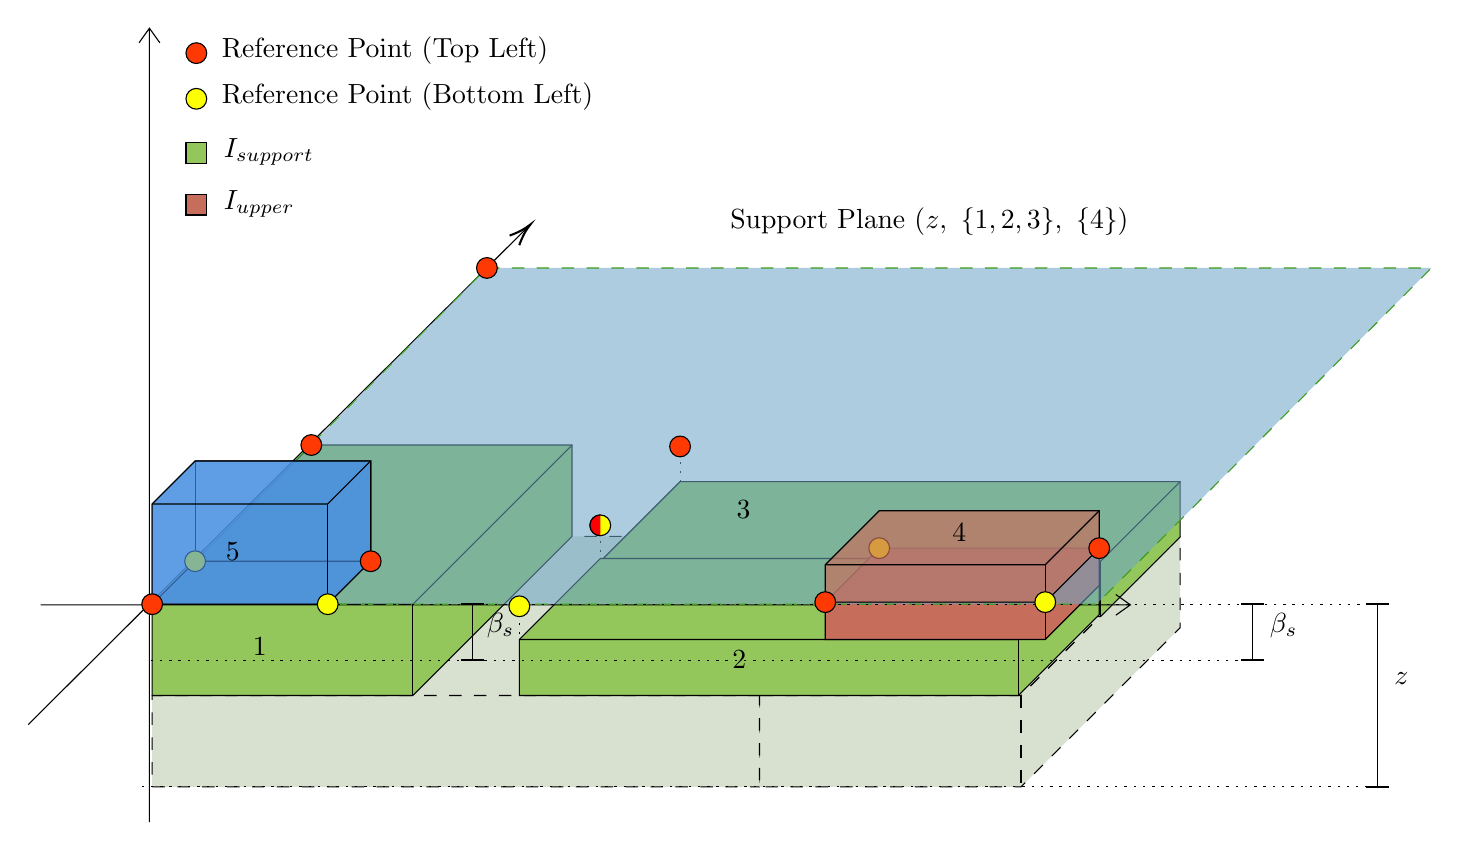
\begin{tikzpicture}[x=0.75pt,y=0.75pt,yscale=-1,xscale=1]
%uncomment if require: \path (0,412); %set diagram left start at 0, and has height of 412

%Shape: Cube [id:dp7106500856615827] 
\draw  [fill={rgb, 255:red, 216; green, 224; blue, 207 }  ,fill opacity=1 ][dash pattern={on 4.5pt off 4.5pt}] (69.7,334.5) -- (146.4,257.81) -- (439,257.81) -- (439,301.81) -- (362.31,378.5) -- (69.7,378.5) -- cycle ; \draw  [dash pattern={on 4.5pt off 4.5pt}] (439,257.81) -- (362.31,334.5) -- (69.7,334.5) ; \draw  [dash pattern={on 4.5pt off 4.5pt}] (362.31,334.5) -- (362.31,378.5) ;
%Straight Lines [id:da8316956251676535] 
\draw  [dash pattern={on 0.84pt off 2.51pt}]  (285.62,269.89) -- (285.62,252.5) ;
%Straight Lines [id:da38384433092333237] 
\draw  [dash pattern={on 0.84pt off 2.51pt}]  (324.05,231.89) -- (324.05,214.5) ;
%Shape: Cube [id:dp47709739603214574] 
\draw  [fill={rgb, 255:red, 216; green, 224; blue, 207 }  ,fill opacity=1 ][dash pattern={on 4.5pt off 4.5pt}] (362.31,334.5) -- (439,257.81) -- (565,257.81) -- (565,301.81) -- (488.31,378.5) -- (362.31,378.5) -- cycle ; \draw  [dash pattern={on 4.5pt off 4.5pt}] (565,257.81) -- (488.31,334.5) -- (362.31,334.5) ; \draw  [dash pattern={on 4.5pt off 4.5pt}] (488.31,334.5) -- (488.31,378.5) ;
%Shape: Cube [id:dp7977002200403227] 
\draw  [fill={rgb, 255:red, 147; green, 198; blue, 91 }  ,fill opacity=1 ] (69.7,290.5) -- (146.4,213.81) -- (272,213.81) -- (272,257.81) -- (195.31,334.5) -- (69.7,334.5) -- cycle ; \draw   (272,213.81) -- (195.31,290.5) -- (69.7,290.5) ; \draw   (195.31,290.5) -- (195.31,334.5) ;
%Shape: Cube [id:dp7121611670665484] 
\draw  [fill={rgb, 255:red, 147; green, 198; blue, 91 }  ,fill opacity=1 ] (285.62,269.89) -- (324.05,231.46) -- (565,231.46) -- (565,258.06) -- (526.56,296.5) -- (285.62,296.5) -- cycle ; \draw   (565,231.46) -- (526.56,269.89) -- (285.62,269.89) ; \draw   (526.56,269.89) -- (526.56,296.5) ;
%Shape: Cube [id:dp604763542929154] 
\draw  [fill={rgb, 255:red, 147; green, 198; blue, 91 }  ,fill opacity=1 ] (246.62,307.5) -- (285.62,268.5) -- (526,268.5) -- (526,295.5) -- (487,334.5) -- (246.62,334.5) -- cycle ; \draw   (526,268.5) -- (487,307.5) -- (246.62,307.5) ; \draw   (487,307.5) -- (487,334.5) ;
%Shape: Axis 2D [id:dp786981943451631] 
\draw  (16,290.81) -- (541,290.81)(68.4,13) -- (68.4,395.5) (534,285.81) -- (541,290.81) -- (534,295.81) (63.4,20) -- (68.4,13) -- (73.4,20)  ;
%Straight Lines [id:da31524103851047525] 
\draw    (10,348.5) -- (250.58,108.91) ;
\draw [shift={(252,107.5)}, rotate = 135.12] [color={rgb, 255:red, 0; green, 0; blue, 0 }  ][line width=0.75]    (10.93,-3.29) .. controls (6.95,-1.4) and (3.31,-0.3) .. (0,0) .. controls (3.31,0.3) and (6.95,1.4) .. (10.93,3.29)   ;
%Shape: Cube [id:dp6424617162036526] 
\draw  [fill={rgb, 255:red, 198; green, 110; blue, 91 }  ,fill opacity=1 ] (394,289.5) -- (420,263.5) -- (526,263.5) -- (526,281.5) -- (500,307.5) -- (394,307.5) -- cycle ; \draw   (526,263.5) -- (500,289.5) -- (394,289.5) ; \draw   (500,289.5) -- (500,307.5) ;
%Shape: Parallelogram [id:dp3639839698249763] 
\draw  [color={rgb, 255:red, 62; green, 156; blue, 30 }  ,draw opacity=1 ][fill={rgb, 255:red, 110; green, 165; blue, 200 }  ,fill opacity=0.57 ][dash pattern={on 4.5pt off 4.5pt}] (231,128.5) -- (686,128.5) -- (524.7,290.5) -- (69.7,290.5) -- cycle ;
%Straight Lines [id:da11997650250706615] 
\draw    (659.96,290.5) -- (659.96,378.5) ;
\draw [shift={(659.96,378.5)}, rotate = 270] [color={rgb, 255:red, 0; green, 0; blue, 0 }  ][line width=0.75]    (0,5.59) -- (0,-5.59)   ;
\draw [shift={(659.96,290.5)}, rotate = 270] [color={rgb, 255:red, 0; green, 0; blue, 0 }  ][line width=0.75]    (0,5.59) -- (0,-5.59)   ;
%Straight Lines [id:da7479086158615895] 
\draw  [dash pattern={on 0.84pt off 2.51pt}]  (69.7,290.5) -- (665,290.5) ;
%Straight Lines [id:da00936893511639092] 
\draw  [dash pattern={on 0.84pt off 2.51pt}]  (64.66,378.5) -- (659.96,378.5) ;
%Straight Lines [id:da2603505755036556] 
\draw  [dash pattern={on 0.84pt off 2.51pt}]  (69,317.5) -- (600,317.5) ;
%Straight Lines [id:da21695403696781168] 
\draw    (600,290.5) -- (600,317.5) ;
\draw [shift={(600,317.5)}, rotate = 270] [color={rgb, 255:red, 0; green, 0; blue, 0 }  ][line width=0.75]    (0,5.59) -- (0,-5.59)   ;
\draw [shift={(600,290.5)}, rotate = 270] [color={rgb, 255:red, 0; green, 0; blue, 0 }  ][line width=0.75]    (0,5.59) -- (0,-5.59)   ;
%Straight Lines [id:da17628222853988207] 
\draw    (224,290.5) -- (224,317.5) ;
\draw [shift={(224,317.5)}, rotate = 270] [color={rgb, 255:red, 0; green, 0; blue, 0 }  ][line width=0.75]    (0,5.59) -- (0,-5.59)   ;
\draw [shift={(224,290.5)}, rotate = 270] [color={rgb, 255:red, 0; green, 0; blue, 0 }  ][line width=0.75]    (0,5.59) -- (0,-5.59)   ;
%Shape: Cube [id:dp458320338188952] 
\draw  [fill={rgb, 255:red, 74; green, 144; blue, 226 }  ,fill opacity=0.66 ] (175,269.8) -- (154.3,290.5) -- (69.7,290.5) -- (69.7,242.2) -- (90.4,221.5) -- (175,221.5) -- cycle ; \draw   (69.7,290.5) -- (90.4,269.8) -- (175,269.8) ; \draw   (90.4,269.8) -- (90.4,221.5) ;
%Shape: Circle [id:dp9728798663710179] 
\draw  [fill={rgb, 255:red, 252; green, 255; blue, 4 }  ,fill opacity=1 ] (86,47) .. controls (86,44.24) and (88.24,42) .. (91,42) .. controls (93.76,42) and (96,44.24) .. (96,47) .. controls (96,49.76) and (93.76,52) .. (91,52) .. controls (88.24,52) and (86,49.76) .. (86,47) -- cycle ;
%Shape: Circle [id:dp41733873180988235] 
\draw  [fill={rgb, 255:red, 252; green, 255; blue, 4 }  ,fill opacity=1 ] (85.4,269.8) .. controls (85.4,267.04) and (87.64,264.8) .. (90.4,264.8) .. controls (93.17,264.8) and (95.4,267.04) .. (95.4,269.8) .. controls (95.4,272.56) and (93.17,274.8) .. (90.4,274.8) .. controls (87.64,274.8) and (85.4,272.56) .. (85.4,269.8) -- cycle ;
%Shape: Cube [id:dp9609158816144449] 
\draw  [fill={rgb, 255:red, 74; green, 144; blue, 226 }  ,fill opacity=0.66 ] (69.7,242.2) -- (90.4,221.5) -- (175,221.5) -- (175,269.8) -- (154.3,290.5) -- (69.7,290.5) -- cycle ; \draw   (175,221.5) -- (154.3,242.2) -- (69.7,242.2) ; \draw   (154.3,242.2) -- (154.3,290.5) ;
%Shape: Circle [id:dp7069570068237806] 
\draw  [fill={rgb, 255:red, 252; green, 255; blue, 4 }  ,fill opacity=1 ] (149.3,290.5) .. controls (149.3,287.74) and (151.54,285.5) .. (154.3,285.5) .. controls (157.06,285.5) and (159.3,287.74) .. (159.3,290.5) .. controls (159.3,293.26) and (157.06,295.5) .. (154.3,295.5) .. controls (151.54,295.5) and (149.3,293.26) .. (149.3,290.5) -- cycle ;
%Shape: Circle [id:dp07493756825553233] 
\draw  [fill={rgb, 255:red, 252; green, 255; blue, 4 }  ,fill opacity=1 ] (241.62,291.5) .. controls (241.62,288.74) and (243.86,286.5) .. (246.62,286.5) .. controls (249.38,286.5) and (251.62,288.74) .. (251.62,291.5) .. controls (251.62,294.26) and (249.38,296.5) .. (246.62,296.5) .. controls (243.86,296.5) and (241.62,294.26) .. (241.62,291.5) -- cycle ;
%Shape: Circle [id:dp9652867077591403] 
\draw  [fill={rgb, 255:red, 252; green, 255; blue, 4 }  ,fill opacity=1 ] (280.62,252.5) .. controls (280.62,249.74) and (282.86,247.5) .. (285.62,247.5) .. controls (288.38,247.5) and (290.62,249.74) .. (290.62,252.5) .. controls (290.62,255.26) and (288.38,257.5) .. (285.62,257.5) .. controls (282.86,257.5) and (280.62,255.26) .. (280.62,252.5) -- cycle ;
%Straight Lines [id:da7143423337159592] 
\draw  [dash pattern={on 0.84pt off 2.51pt}]  (246.62,313.89) -- (246.62,296.5) ;
%Shape: Rectangle [id:dp672375593139905] 
\draw  [fill={rgb, 255:red, 147; green, 198; blue, 91 }  ,fill opacity=1 ] (86,68) -- (96,68) -- (96,78) -- (86,78) -- cycle ;
%Shape: Rectangle [id:dp16133242915286994] 
\draw  [fill={rgb, 255:red, 198; green, 110; blue, 91 }  ,fill opacity=1 ] (86,93) -- (96,93) -- (96,103) -- (86,103) -- cycle ;
%Shape: Circle [id:dp7335317400317659] 
\draw  [fill={rgb, 255:red, 255; green, 57; blue, 4 }  ,fill opacity=1 ] (86,25) .. controls (86,22.24) and (88.24,20) .. (91,20) .. controls (93.76,20) and (96,22.24) .. (96,25) .. controls (96,27.76) and (93.76,30) .. (91,30) .. controls (88.24,30) and (86,27.76) .. (86,25) -- cycle ;
%Shape: Circle [id:dp4790782266696906] 
\draw  [fill={rgb, 255:red, 255; green, 57; blue, 4 }  ,fill opacity=1 ] (319.05,214.5) .. controls (319.05,211.74) and (321.29,209.5) .. (324.05,209.5) .. controls (326.82,209.5) and (329.05,211.74) .. (329.05,214.5) .. controls (329.05,217.26) and (326.82,219.5) .. (324.05,219.5) .. controls (321.29,219.5) and (319.05,217.26) .. (319.05,214.5) -- cycle ;
%Shape: Circle [id:dp3675058769915285] 
\draw  [fill={rgb, 255:red, 255; green, 57; blue, 4 }  ,fill opacity=1 ] (141.4,213.81) .. controls (141.4,211.05) and (143.63,208.81) .. (146.4,208.81) .. controls (149.16,208.81) and (151.4,211.05) .. (151.4,213.81) .. controls (151.4,216.57) and (149.16,218.81) .. (146.4,218.81) .. controls (143.63,218.81) and (141.4,216.57) .. (141.4,213.81) -- cycle ;
%Shape: Circle [id:dp6836568323907531] 
\draw  [fill={rgb, 255:red, 255; green, 57; blue, 4 }  ,fill opacity=1 ] (170,269.8) .. controls (170,267.04) and (172.24,264.8) .. (175,264.8) .. controls (177.76,264.8) and (180,267.04) .. (180,269.8) .. controls (180,272.56) and (177.76,274.8) .. (175,274.8) .. controls (172.24,274.8) and (170,272.56) .. (170,269.8) -- cycle ;
%Shape: Circle [id:dp9319287698621804] 
\draw  [fill={rgb, 255:red, 255; green, 57; blue, 4 }  ,fill opacity=1 ] (64.7,290.5) .. controls (64.7,287.74) and (66.94,285.5) .. (69.7,285.5) .. controls (72.47,285.5) and (74.7,287.74) .. (74.7,290.5) .. controls (74.7,293.26) and (72.47,295.5) .. (69.7,295.5) .. controls (66.94,295.5) and (64.7,293.26) .. (64.7,290.5) -- cycle ;
%Shape: Arc [id:dp7222867806291037] 
\draw  [draw opacity=0][fill={rgb, 255:red, 251; green, 1; blue, 1 }  ,fill opacity=1 ] (285.62,257.5) .. controls (285.62,257.5) and (285.62,257.5) .. (285.62,257.5) .. controls (285.62,257.5) and (285.62,257.5) .. (285.62,257.5) .. controls (282.86,257.5) and (280.62,255.26) .. (280.62,252.5) .. controls (280.62,249.74) and (282.86,247.5) .. (285.62,247.5) -- (285.62,252.5) -- cycle ; \draw   (285.62,257.5) .. controls (285.62,257.5) and (285.62,257.5) .. (285.62,257.5) .. controls (285.62,257.5) and (285.62,257.5) .. (285.62,257.5) .. controls (282.86,257.5) and (280.62,255.26) .. (280.62,252.5) .. controls (280.62,249.74) and (282.86,247.5) .. (285.62,247.5) ;  
%Shape: Circle [id:dp7431470261343242] 
\draw  [fill={rgb, 255:red, 252; green, 255; blue, 4 }  ,fill opacity=1 ] (415,263.5) .. controls (415,260.74) and (417.24,258.5) .. (420,258.5) .. controls (422.76,258.5) and (425,260.74) .. (425,263.5) .. controls (425,266.26) and (422.76,268.5) .. (420,268.5) .. controls (417.24,268.5) and (415,266.26) .. (415,263.5) -- cycle ;
%Shape: Cube [id:dp46874066075395426] 
\draw  [fill={rgb, 255:red, 198; green, 110; blue, 91 }  ,fill opacity=0.69 ] (394,271.5) -- (420,245.5) -- (526,245.5) -- (526,263.5) -- (500,289.5) -- (394,289.5) -- cycle ; \draw   (526,245.5) -- (500,271.5) -- (394,271.5) ; \draw   (500,271.5) -- (500,289.5) ;
%Shape: Circle [id:dp4546060900911436] 
\draw  [fill={rgb, 255:red, 252; green, 255; blue, 4 }  ,fill opacity=1 ] (495,289.5) .. controls (495,286.74) and (497.24,284.5) .. (500,284.5) .. controls (502.76,284.5) and (505,286.74) .. (505,289.5) .. controls (505,292.26) and (502.76,294.5) .. (500,294.5) .. controls (497.24,294.5) and (495,292.26) .. (495,289.5) -- cycle ;
%Shape: Circle [id:dp1099531157368071] 
\draw  [fill={rgb, 255:red, 255; green, 57; blue, 4 }  ,fill opacity=1 ] (521,263.5) .. controls (521,260.74) and (523.24,258.5) .. (526,258.5) .. controls (528.76,258.5) and (531,260.74) .. (531,263.5) .. controls (531,266.26) and (528.76,268.5) .. (526,268.5) .. controls (523.24,268.5) and (521,266.26) .. (521,263.5) -- cycle ;
%Shape: Circle [id:dp6477599340697807] 
\draw  [fill={rgb, 255:red, 255; green, 57; blue, 4 }  ,fill opacity=1 ] (389,289.5) .. controls (389,286.74) and (391.24,284.5) .. (394,284.5) .. controls (396.76,284.5) and (399,286.74) .. (399,289.5) .. controls (399,292.26) and (396.76,294.5) .. (394,294.5) .. controls (391.24,294.5) and (389,292.26) .. (389,289.5) -- cycle ;
%Shape: Circle [id:dp38665130344221843] 
\draw  [fill={rgb, 255:red, 255; green, 57; blue, 4 }  ,fill opacity=1 ] (226,128.5) .. controls (226,125.74) and (228.24,123.5) .. (231,123.5) .. controls (233.76,123.5) and (236,125.74) .. (236,128.5) .. controls (236,131.26) and (233.76,133.5) .. (231,133.5) .. controls (228.24,133.5) and (226,131.26) .. (226,128.5) -- cycle ;

% Text Node
\draw (667,322.4) node [anchor=north west][inner sep=0.75pt]    {$z$};
% Text Node
\draw (347,98) node [anchor=north west][inner sep=0.75pt]   [align=left] {Support Plane $\displaystyle ( z,\ \{1,2,3\} ,\ \{4\})$};
% Text Node
\draw (104,259.4) node [anchor=north west][inner sep=0.75pt]    {$5$};
% Text Node
\draw (117,305.4) node [anchor=north west][inner sep=0.75pt]    {$1$};
% Text Node
\draw (348,311.4) node [anchor=north west][inner sep=0.75pt]    {$2$};
% Text Node
\draw (350,239.4) node [anchor=north west][inner sep=0.75pt]    {$3$};
% Text Node
\draw (454,250.4) node [anchor=north west][inner sep=0.75pt]    {$4$};
% Text Node
\draw (607,293.4) node [anchor=north west][inner sep=0.75pt]    {$\beta _{s}$};
% Text Node
\draw (229.67,293.4) node [anchor=north west][inner sep=0.75pt]    {$\beta _{s}$};
% Text Node
\draw (102,38) node [anchor=north west][inner sep=0.75pt]   [align=left] {Reference Point (Bottom Left)};
% Text Node
\draw (103,65) node [anchor=north west][inner sep=0.75pt]   [align=left] {$\displaystyle I_{support}$};
% Text Node
\draw (103,90) node [anchor=north west][inner sep=0.75pt]   [align=left] {$\displaystyle I_{upper}$};
% Text Node
\draw (102,16) node [anchor=north west][inner sep=0.75pt]   [align=left] {Reference Point (Top Left)};


\end{tikzpicture}

    }
    \caption{Representation of a generic support plane with a placed item}
    \label{fig:support_planes}
\end{figure}

\begin{figure}[hp]
    \centering
    %\scalebox{0.75}{%
    

\tikzset{every picture/.style={line width=0.75pt}} %set default line width to 0.75pt        

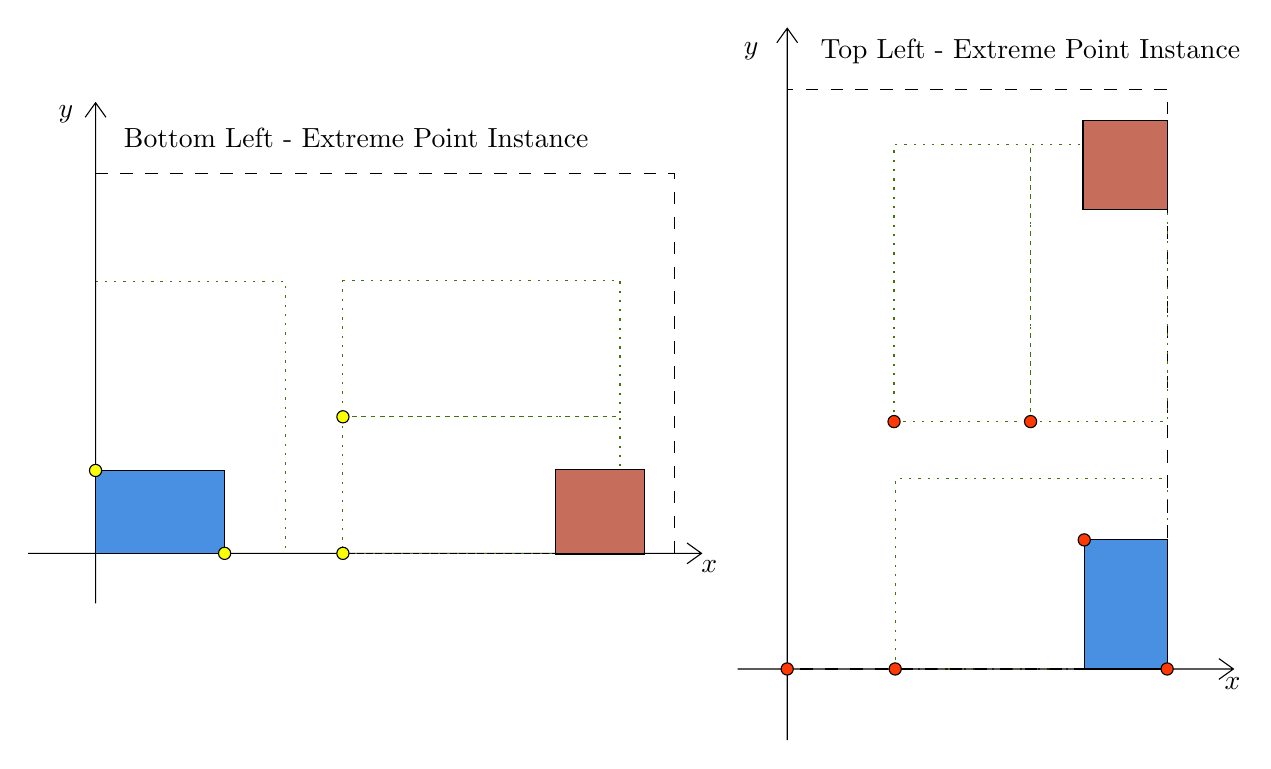
\begin{tikzpicture}[x=0.75pt,y=0.75pt,yscale=-1,xscale=1]
%uncomment if require: \path (0,380); %set diagram left start at 0, and has height of 380

%Shape: Rectangle [id:dp676391404304541] 
\draw  [color={rgb, 255:red, 65; green, 117; blue, 5 }  ,draw opacity=1 ][dash pattern={on 0.84pt off 2.51pt}] (65.44,151.69) -- (157,151.69) -- (157,282.71) -- (65.44,282.71) -- cycle ;
%Shape: Rectangle [id:dp26001178837889305] 
\draw  [color={rgb, 255:red, 65; green, 117; blue, 5 }  ,draw opacity=1 ][dash pattern={on 0.84pt off 2.51pt}] (450.7,338.41) -- (450.7,246.85) -- (581.72,246.85) -- (581.72,338.41) -- cycle ;
%Shape: Rectangle [id:dp532870934725963] 
\draw  [dash pattern={on 4.5pt off 4.5pt}] (65.44,99.66) -- (344.58,99.66) -- (344.58,282.71) -- (65.44,282.71) -- cycle ;
%Shape: Axis 2D [id:dp545947560183275] 
\draw  (33,282.71) -- (357.39,282.71)(65.44,65.6) -- (65.44,306.84) (350.39,277.71) -- (357.39,282.71) -- (350.39,287.71) (60.44,72.6) -- (65.44,65.6) -- (70.44,72.6)  ;
%Shape: Rectangle [id:dp13640021794487145] 
\draw  [fill={rgb, 255:red, 74; green, 144; blue, 226 }  ,fill opacity=1 ] (65.44,242.78) -- (127.61,242.78) -- (127.61,282.71) -- (65.44,282.71) -- cycle ;
%Shape: Ellipse [id:dp4997787088203596] 
\draw  [fill={rgb, 255:red, 252; green, 255; blue, 4 }  ,fill opacity=1 ] (62.5,242.78) .. controls (62.5,241.16) and (63.82,239.84) .. (65.44,239.84) .. controls (67.06,239.84) and (68.38,241.16) .. (68.38,242.78) .. controls (68.38,244.4) and (67.06,245.72) .. (65.44,245.72) .. controls (63.82,245.72) and (62.5,244.4) .. (62.5,242.78) -- cycle ;
%Shape: Ellipse [id:dp9368091558454169] 
\draw  [fill={rgb, 255:red, 252; green, 255; blue, 4 }  ,fill opacity=1 ] (124.67,282.71) .. controls (124.67,281.09) and (125.99,279.77) .. (127.61,279.77) .. controls (129.24,279.77) and (130.55,281.09) .. (130.55,282.71) .. controls (130.55,284.34) and (129.24,285.65) .. (127.61,285.65) .. controls (125.99,285.65) and (124.67,284.34) .. (124.67,282.71) -- cycle ;
%Shape: Rectangle [id:dp10130767347226488] 
\draw  [color={rgb, 255:red, 65; green, 117; blue, 5 }  ,draw opacity=1 ][dash pattern={on 0.84pt off 2.51pt}] (184.62,216.92) -- (318.13,216.92) -- (318.13,282.71) -- (184.62,282.71) -- cycle ;
%Shape: Rectangle [id:dp8859988076373574] 
\draw  [color={rgb, 255:red, 65; green, 117; blue, 5 }  ,draw opacity=1 ][dash pattern={on 0.84pt off 2.51pt}] (184.62,151.14) -- (318.13,151.14) -- (318.13,216.92) -- (184.62,216.92) -- cycle ;
%Shape: Rectangle [id:dp5346376956315015] 
\draw  [fill={rgb, 255:red, 198; green, 110; blue, 91 }  ,fill opacity=1 ] (286.87,242.19) -- (329.77,242.19) -- (329.77,283.04) -- (286.87,283.04) -- cycle ;
%Shape: Ellipse [id:dp5380867242688693] 
\draw  [fill={rgb, 255:red, 252; green, 255; blue, 4 }  ,fill opacity=1 ] (181.68,282.71) .. controls (181.68,281.09) and (182.99,279.77) .. (184.62,279.77) .. controls (186.24,279.77) and (187.55,281.09) .. (187.55,282.71) .. controls (187.55,284.34) and (186.24,285.65) .. (184.62,285.65) .. controls (182.99,285.65) and (181.68,284.34) .. (181.68,282.71) -- cycle ;
%Shape: Circle [id:dp32824759445274065] 
\draw  [fill={rgb, 255:red, 252; green, 255; blue, 4 }  ,fill opacity=1 ] (181.68,216.92) .. controls (181.68,215.3) and (182.99,213.99) .. (184.62,213.99) .. controls (186.24,213.99) and (187.55,215.3) .. (187.55,216.92) .. controls (187.55,218.55) and (186.24,219.86) .. (184.62,219.86) .. controls (182.99,219.86) and (181.68,218.55) .. (181.68,216.92) -- cycle ;
%Shape: Rectangle [id:dp013806976369067359] 
\draw  [dash pattern={on 4.5pt off 4.5pt}] (398.67,338.41) -- (398.67,59.27) -- (581.72,59.27) -- (581.72,338.41) -- cycle ;
%Shape: Axis 2D [id:dp26544149420697416] 
\draw  (374.78,338.41) -- (613.65,338.41)(398.67,29.71) -- (398.67,372.71) (606.65,333.41) -- (613.65,338.41) -- (606.65,343.41) (393.67,36.71) -- (398.67,29.71) -- (403.67,36.71)  ;
%Shape: Rectangle [id:dp4452985784509189] 
\draw  [fill={rgb, 255:red, 74; green, 144; blue, 226 }  ,fill opacity=1 ] (541.79,338.41) -- (541.79,276.23) -- (581.72,276.23) -- (581.72,338.41) -- cycle ;
%Shape: Rectangle [id:dp24524128214266327] 
\draw  [color={rgb, 255:red, 65; green, 117; blue, 5 }  ,draw opacity=1 ][dash pattern={on 0.84pt off 2.51pt}] (515.93,219.23) -- (515.93,85.71) -- (581.72,85.71) -- (581.72,219.23) -- cycle ;
%Shape: Rectangle [id:dp5234703657507643] 
\draw  [color={rgb, 255:red, 65; green, 117; blue, 5 }  ,draw opacity=1 ][dash pattern={on 0.84pt off 2.51pt}] (450.14,219.23) -- (450.14,85.71) -- (515.93,85.71) -- (515.93,219.23) -- cycle ;
%Shape: Rectangle [id:dp9419058705222738] 
\draw  [fill={rgb, 255:red, 198; green, 110; blue, 91 }  ,fill opacity=1 ] (541.2,116.98) -- (541.2,74.08) -- (582.04,74.08) -- (582.04,116.98) -- cycle ;
%Shape: Ellipse [id:dp3331578572136539] 
\draw  [fill={rgb, 255:red, 255; green, 57; blue, 4 }  ,fill opacity=1 ] (450.14,222.17) .. controls (448.52,222.17) and (447.21,220.85) .. (447.21,219.23) .. controls (447.21,217.61) and (448.52,216.29) .. (450.14,216.29) .. controls (451.77,216.29) and (453.08,217.61) .. (453.08,219.23) .. controls (453.08,220.85) and (451.77,222.17) .. (450.14,222.17) -- cycle ;
%Shape: Ellipse [id:dp23570925769851603] 
\draw  [fill={rgb, 255:red, 255; green, 57; blue, 4 }  ,fill opacity=1 ] (515.93,222.17) .. controls (514.31,222.17) and (512.99,220.85) .. (512.99,219.23) .. controls (512.99,217.61) and (514.31,216.29) .. (515.93,216.29) .. controls (517.56,216.29) and (518.87,217.61) .. (518.87,219.23) .. controls (518.87,220.85) and (517.56,222.17) .. (515.93,222.17) -- cycle ;
%Shape: Ellipse [id:dp6429169005498813] 
\draw  [fill={rgb, 255:red, 255; green, 57; blue, 4 }  ,fill opacity=1 ] (398.67,341.35) .. controls (397.04,341.35) and (395.73,340.03) .. (395.73,338.41) .. controls (395.73,336.78) and (397.04,335.47) .. (398.67,335.47) .. controls (400.29,335.47) and (401.6,336.78) .. (401.6,338.41) .. controls (401.6,340.03) and (400.29,341.35) .. (398.67,341.35) -- cycle ;
%Shape: Ellipse [id:dp5636473664839672] 
\draw  [fill={rgb, 255:red, 255; green, 57; blue, 4 }  ,fill opacity=1 ] (450.7,341.35) .. controls (449.08,341.35) and (447.76,340.03) .. (447.76,338.41) .. controls (447.76,336.78) and (449.08,335.47) .. (450.7,335.47) .. controls (452.33,335.47) and (453.64,336.78) .. (453.64,338.41) .. controls (453.64,340.03) and (452.33,341.35) .. (450.7,341.35) -- cycle ;
%Shape: Ellipse [id:dp310194773919646] 
\draw  [fill={rgb, 255:red, 255; green, 57; blue, 4 }  ,fill opacity=1 ] (581.72,341.35) .. controls (580.1,341.35) and (578.78,340.03) .. (578.78,338.41) .. controls (578.78,336.78) and (580.1,335.47) .. (581.72,335.47) .. controls (583.34,335.47) and (584.66,336.78) .. (584.66,338.41) .. controls (584.66,340.03) and (583.34,341.35) .. (581.72,341.35) -- cycle ;
%Shape: Ellipse [id:dp4413085834987862] 
\draw  [fill={rgb, 255:red, 255; green, 57; blue, 4 }  ,fill opacity=1 ] (541.79,279.17) .. controls (540.17,279.17) and (538.85,277.86) .. (538.85,276.23) .. controls (538.85,274.61) and (540.17,273.29) .. (541.79,273.29) .. controls (543.41,273.29) and (544.73,274.61) .. (544.73,276.23) .. controls (544.73,277.86) and (543.41,279.17) .. (541.79,279.17) -- cycle ;

% Text Node
\draw (46.39,65.64) node [anchor=north west][inner sep=0.75pt]    {$y$};
% Text Node
\draw (356.09,284.84) node [anchor=north west][inner sep=0.75pt]    {$x$};
% Text Node
\draw (77.86,76.79) node [anchor=north west][inner sep=0.75pt]   [align=left] {Bottom Left - Extreme Point Instance};
% Text Node
\draw (376.52,35.3) node [anchor=north west][inner sep=0.75pt]    {$y$};
% Text Node
\draw (608.21,341.49) node [anchor=north west][inner sep=0.75pt]    {$x$};
% Text Node
\draw (413.49,33.94) node [anchor=north west][inner sep=0.75pt]   [align=left] {Top Left - Extreme Point Instance};


\end{tikzpicture}

    %}
    \caption{Extreme Point instances for some coordinate changes of \cref{fig:support_planes}}
    \label{fig:ep_coordinate_changes}
\end{figure}

Given \cref{eq:ep_can_pack} to check if a considered placement would lead to a feasible insertion, a set of items to pack $I$, a set $s$ and a bin $b \in B^s$, the heuristic that will output the new best possible feasible insertion for the given set of items is outlined in Algo. \ref{algo:sp_bestinsertion}.

\begin{algorithm}[hp]
    \DontPrintSemicolon
    \SetAlgoLined
    \SetKwInOut{Input}{input}
    \SetKwInOut{Output}{output}
    \Input{$Z, I, T$}
    \Output{$p$}
    \ForAll{$(z, I_{support}, I_{upper}) \in Z$}{
        $P \gets \emptyset$\;
        \ForAll{possible coordinate changes}{
            $p \leftarrow (z, \emptyset)$\;
            $T^\prime \gets \text{empty AABB tree}$\;
            \CommentSty{//Initialize reference points}\;
            $refPoints \gets (0,0)$\;
            \ForAll{$i \in I_{support}$}{
                $refPoints \gets refPoints \cup \{(x_i, y_i)\}$\;
            }
            \ForAll{$i \in I_{upper}$}{
                $refPoints \gets refPoints \cup \{(x_i + w_i, y_i), (x_i, y_i + d_i)\}$\;
            }
            $sort(refPoints)$ \CommentSty{// Based on euclidean distance from $(0,0)$}\;

            \CommentSty{//Create a feasible insertion for the given items}\;
            \ForAll{$i \in I$}{
                \CommentSty{//Evaluate first possible placement}\;
                \ForAll{$(x,y) \in refPoints$}{
                    $(x_i, y_i, z_i) \gets (x, y, z)$\;
                    \If{$EPCanPlace(i, T, T^\prime)$}{
                        $EPInsertRect(p, i, T^\prime, refPoints)$ \CommentSty{// alg. \ref{algo:ep_insert_rect}}\;
                        break\;
                    }
                    $(w_i, d_i) \gets (d_i, w_i)$ \CommentSty{//Try rotating $i$}\;
                    \If{$EPCanPlace(i, T, T^\prime)$}{
                        $EPInsertRect(p, i, T^\prime, refPoints)$ \CommentSty{// alg. \ref{algo:ep_insert_rect}}\;
                        break\;
                    }
                    $(w_i, d_i) \gets (d_i, w_i)$ \CommentSty{//Restore original $i$ rotation}\;
                }
            }
            \If{$p \neq (z, \emptyset)$}{
                $P \gets P \cup \{ p \}$\;
            }
        }
        $sort(P)$ \CommentSty{//Sorted as in \cref{ssec:scoring_insertions}}\;
        \If{$P \neq \emptyset$}{
            \Return{first element of $P$}
        }
    }
    \Return{none}
    \caption{SP Best Insertion \label{algo:sp_bestinsertion}}
\end{algorithm}
\begin{algorithm}[htb] 
    \DontPrintSemicolon
    \SetAlgoLined
    \SetKwInOut{Input}{input}
    \SetKwInOut{Output}{output}
    \Input{ $p, i, T, refPoints$}
    $refPoints \gets refPoints \setminus \{ (x_i, y_i) \}$\;
    $refPoints \gets refPoints \cup \{(x_i + w_i, y_i), (x_i, y_i + d_i)\}$\;
    $sort(refPoints)$ \CommentSty{// Based on euclidean distance from $(0,0)$}\;
    $p.I \gets p.I \cup \{ i \}$\;
    $AABBInsert(i, T^\prime)$ \CommentSty{//\cref{sec:problem_state:aabbtree}}\;
    \Return
    \caption{EP Insert Rect \label{algo:ep_insert_rect}}
\end{algorithm}

\paragraph*{Commit Extension}
We now describe an extension to $Commit$ (Algo. \ref{algo:state_commit}) that updates the structures needed by SP.

When a plane is filled, new insertions become less likely to be feasible.
To avoid evaluating planes where no insertion is possible we develop a mechanism to prune dead planes.

Since best insertions for a bin are always evaluated by considering lower planes first, if all the insertions in $Expand$ (Algo. \ref{algo:state_successor}) happened over a $z_{min}$, then we can safely remove the opened planes with $z < z_{min}$ for that bin.
Let us introduce a $z^s_{min}$ variable that is updated during the $Expand$ phase with the minimum $z$ of all the insertions on bin $b$.
Once the best states are computed and $Commit$ is called, we can use $z^s_{min}$ to prune planes in each $b \in B^s$.
Other operations are also necessary in the $Commit$ algorithm to allow SP to update its data structures accordingly to the insertion.

Let $s$ be a state and let $p$ be an insertion where each packed item $i \in I_p$ in bin $b_p$ has $z^s_i$ within tolerance of $z$.
The algorithm which updates the structures for a given bin $b$ is represented by algorithm \ref{algo:sp_commit}.
This new algorithm can be used as the last step of the $Commit$ algorithm for each $b \in B^{s^\prime}$.

\begin{algorithm}[H] \label{algo:sp_commit}
    \DontPrintSemicolon
    \SetAlgoLined
    \SetKwInOut{Input}{input}
    \SetKwInOut{Output}{output}
    \SetSideCommentRight
    \Input{$s_b, I, z, z_{min}, t$}
    \Output{$s^\prime_b$}
    \CommentSty{//Filter bad planes}\;
    $P^\prime \leftarrow planes \setminus \{ \forall S_z \in planes : z \le z_{min} \}$\;
    \CommentSty{//Apply insertion}\;
    $B \leftarrow placed \cup I$\;
    $U \leftarrow unpacked \setminus I$\;
    $T \leftarrow aabb$\;
    \ForAll{$i \in I$}{
        $T \leftarrow InsertAABB(i, T)$ \CommentSty{//If balanced $O(log(n))$}\; %TODO: specify balanced
        $generate \leftarrow true$\;
        % O(|P'|)
        \ForAll{$S^\prime_z \in P^\prime$}{ %TODO: specify balanced
            \CommentSty{//Based on the distance from the top of the item}\;
            $dz \leftarrow S^\prime_z.z - i.z_{max}$\;
            \If{$0 \le dz \le t$}{
                $generate \leftarrow false$\;
                $S^\prime_z.I_{support} \leftarrow S^\prime_z.I_{support} \cup i$\;
            } \ElseIf{$dz < 0$}{
                $S^\prime_z.I_{upper} \leftarrow S^\prime_z.I_{upper} \cup i$\;
            }
        }

        \If{$generate$}{
            $P^\prime \leftarrow P^\prime \cup (i.z_{max}, \{i\}, \emptyset)$\;
        }
    }
    \Return{$Update(s_b, P^\prime, B, U, T)$}
    \caption{SP Apply and Filter}
\end{algorithm}

\subsection{Ranking Insertions}
\label{ssec:scoring_insertions}%
Similarly to the ranking of states (\cref{ssec:scoring_states}), an ordering function is also needed to evaluate different insertions for the same set of items.
Given the lexicographic ordering formulation in \cref{def:lexicographic_ordering}, a few new functions can be calculated and stored inside an insertion to help in the evaluation.
Given $T$ as the AABB Tree that represents the bin where the insertion is going to happen, and given one of the inserted items $i \in I_p$, we define functions that use the tree to calculate useful metrics:
\begin{itemize}
    \item $CloseItems(i, T)$: which returns the number of packed items that are close to $i$,
    \item $CloseSameHeight(i, T)$: which returns the number of packed items in the tree that are close to $i$ and with its same height,
    \item $CloseSameShape(i, T)$: which returns the number of packed items in the tree that are close to $i$ and with its same shape,
    \item $TotalSupportedArea(i, T)$: which returns the total base area of $i$ which is supported by other items.
\end{itemize}
We then sort insertions $p$, given $T$ as the AABB tree of the bin where the insertion will happen, with a lexicographic ordering as follows:
\begin{itemize}
    \item $f_1(p) = -\sum\limits_{i \in I_p}{CloseSameShape(i, T)} - |I_p|$: maximize number of items inserted (of the same shape) that are close to already packed items of the same shape,
    \item $f_2(p) = -\sum\limits_{i \in I_p}{(w^s_i d^s_i + w^s_i d^s_i h^s_i)}$: maximize the sum of the area and volume of each packed item,
    \item $f_3(p) = \max\limits_{i \in I_p}(z^s_i + h_i)$: minimize the maximum height of the inserted items,
    \item $f_4(p) = \sum\limits_{i \in I_p}{TotalSupportedArea(i, T)}$: minimize the support area available to the inserted items,
    \item $f_5(p) = -\sum\limits_{i \in I_p}{CloseSameHeight(i, T)} - |I_p|$: maximize the number of items inserted (of the same height) that are close to already packed items of the same height,
    \item $f_5(p) = -\sum\limits_{i \in I_p}{CloseItems(i, T)} - |I_p|$: maximize the number of items inserted that are close to already packed items.
\end{itemize}
We note that preferring feasible insertions that minimize the supported area of each item as in $f_4$ is inspired by other works on spacing from the literature.
As shown in \cite{elhedhli2019three}, overly satisfying the support constraint can lead to unbalanced bins.
Minimizing the supported area of each item leads to minimizing the perimeter of overlap between items which in turn results in more balanced bins that have better spacing between items.

    \chapter{Computational experiments}
    \label{chapther:experiments}%
    In this chapter, in \cref{exp:model_tests}, we evaluate the proposed heuristic against the MILP model (\ref{sec:milp}), and in \cref{exp:literature_tests} against other heuristics from the literature. We then show the effectiveness of our approach for our case study in \cref{exp:usecase_results}.
All the tests were run on a desktop computer with an AMD Ryzen-7 5800x processor with 8 cores at 3.8 GHz and 32GB of DDR4 system RAM with Windows 10. The algorithm was implemented in Java 11, and the model was run using the python APIs from CPLEX Optimization Studio 22.1.0.
In every test, CPLEX was used with a maximum runtime of 1 hour.
Each evaluation against the heuristic lists both operational modes described in \cref{def:placement_modes} listed as "PM" and "PS".
All the instances used in each section of this chapter are available at \url{https://github.com/artumino/BinPackingThesis/tree/main/tests/instances}.
Out of the 100 instances used for our case study experiments, only 80 were freely sharable with the generation procedure also described in \cref{exp:usecase_results}.

\section{Model validation}
We compared our heuristic to the proposed MILP model of \cref{sec:milp} with a single bin and with no limit on the height of the bin (also referred to as the 3D strip packing problem).
The heuristic was configured to run without vertex support, using only area support rules for its feasibility checks, and $k$ was set to $200$.
The configured parameters for the test were $\alpha_s = 0.7$, $\beta_s = 5$, and the discretization unit for the model was $\delta = 10$.
Tests were run on the first generated instance of the class 1 problems from \citep{martello2000three} which we used for literature tests. These classes of problem have a bin base of $100 \times 100$.
The test were run with an iterative approach by selecting only a limited amount of items from the selected instance, starting from the first item and increasing the number of items to pack by one at each iteration.
The problem created with each iteration was saved as a test instance in the same format as the one used for literature tests.
All the generated instances are available at \url{https://github.com/artumino/BinPackingThesis/tree/main/tests/instances/model}.
A python script then loaded each generated instance sequentially and evaluated the solutions from both the MILP problem and the heuristic. %FIXME: Describe python script
Starting from instance 6, the solution from the previous instance was used to mip start the new one leading to lower execution times.

Table \ref{exp:model} shows the obtained $z_{\text{max}}$ value of the heuristic and the MILP solution, the runtime in seconds, and the number of items.
Since the underlying problem is NP-Hard, it is shown that starting from instances of size bigger than 8 items; the MILP model becomes too slow for practical use while our heuristic maintains negligible execution time.
Due to discretization errors, some of the model instances gave solutions that didn't have the expected amount of support and were marked with an asterisk.
The solution to instance number 5 and instance number 7 is also shown in \cref{fig:model_tests}.
\label{exp:model_tests}
\begin{table}[htbp]
    \centering
    \caption{Comparison with MILP model on limited set of boxes}
    \begin{tabular}{|c|c|c|c|c|c|c|c|}
    \hline
    & \multicolumn{ 3}{c|}{\textbf{MILP Model}} & \multicolumn{ 2}{c|}{\textbf{PM}} & \multicolumn{ 2}{c|}{\textbf{PS}} \\ \hline
    \textbf{$n$} & \textbf{Max Z} & \textbf{TT(s)} & \textbf{Gap($\%$)} & \textbf{Max Z} & \textbf{TT(s)} & \textbf{Max Z} & \textbf{TT(s)} \\ \hline
    1  & 85   & 0.01     & 0.00 & 85  & 0.00 & 85  & 0.00 \\ 
    2  & 85   & 0.07     & 0.00 & 85  & 0.00 & 85  & 0.00 \\ 
    3  & 85   & 0.13     & 0.00 & 85  & 0.00 & 85  & 0.00 \\ 
    4  & 85   & 0.20     & 0.00 & 85  & 0.01 & 85  & 0.01 \\ 
    5  & 85   & 2.02     & 0.00 & 85  & 0.02 & 85  & 0.02 \\ 
    6  & 158  & 90.58    & 0.00 & 158 & 0.06 & 158 & 0.05 \\ 
    7  & 158  & 1,369.24 & 0.00 & 158 & 0.07 & 158 & 0.08 \\ 
    8  & 161* & 3,600.00 & 1.86 & 160 & 0.10 & 160 & 0.08 \\ \hline
    9  & -    & -        & -    & 169 & 0.09 & 161 & 0.10 \\ 
    10 & -    & -        & -    & 218 & 0.12 & 218 & 0.13 \\ 
    11 & -    & -        & -    & 240 & 0.12 & 240 & 0.12 \\ 
    12 & -    & -        & -    & 310 & 0.13 & 316 & 0.16 \\ 
    13 & -    & -        & -    & 310 & 0.15 & 333 & 0.18 \\ 
    14 & -    & -        & -    & 310 & 0.20 & 333 & 0.22 \\ 
    15 & -    & -        & -    & 406 & 0.21 & 397 & 0.27 \\ 
    16 & -    & -        & -    & 435 & 0.23 & 452 & 0.36 \\ 
    17 & -    & -        & -    & 429 & 0.27 & 515 & 0.41 \\ 
    18 & -    & -        & -    & 432 & 0.32 & 522 & 0.47 \\ 
    19 & -    & -        & -    & 458 & 0.35 & 522 & 0.55 \\ 
    20 & -    & -        & -    & 539 & 0.37 & 564 & 0.62 \\ \hline
    \end{tabular}
    \label{exp:model}
    \caption*{* Some boxes had lower support than expected due to discretization errors.}
    \end{table}

\begin{table}[htbp]
    \centering
    \caption{Comparison with MILP model on limited set of boxes}
    \begin{tabular}{|c|c|c|c|c|c|c|c|}
    \hline
    & \multicolumn{ 3}{c|}{\textbf{MILP Model}} & \multicolumn{ 2}{c|}{\textbf{PM}} & \multicolumn{ 2}{c|}{\textbf{PS}} \\ \hline
    \textbf{$n$} & \textbf{Max Z} & \textbf{TT(s)} & \textbf{Gap($\%$)} & \textbf{Max Z} & \textbf{TT(s)} & \textbf{Max Z} & \textbf{TT(s)} \\ \hline
    1  & 85   & 0.01     & 0.00 & 85  & 0.00 & 85  & 0.00 \\ 
    2  & 85   & 0.07     & 0.00 & 85  & 0.00 & 85  & 0.00 \\ 
    3  & 85   & 0.13     & 0.00 & 85  & 0.00 & 85  & 0.00 \\ 
    4  & 85   & 0.20     & 0.00 & 85  & 0.01 & 85  & 0.01 \\ 
    5  & 85   & 2.02     & 0.00 & 85  & 0.02 & 85  & 0.02 \\ 
    6  & 158  & 90.58    & 0.00 & 158 & 0.06 & 158 & 0.05 \\ 
    7  & 158  & 1,369.24 & 0.00 & 158 & 0.07 & 158 & 0.08 \\ 
    8  & 161* & 3,600.00 & 1.86 & 160 & 0.10 & 160 & 0.08 \\ \hline
    9  & -    & -        & -    & 169 & 0.09 & 161 & 0.10 \\ 
    10 & -    & -        & -    & 218 & 0.12 & 218 & 0.13 \\ 
    11 & -    & -        & -    & 240 & 0.12 & 240 & 0.12 \\ 
    12 & -    & -        & -    & 310 & 0.13 & 316 & 0.16 \\ 
    13 & -    & -        & -    & 310 & 0.15 & 333 & 0.18 \\ 
    14 & -    & -        & -    & 310 & 0.20 & 333 & 0.22 \\ 
    15 & -    & -        & -    & 406 & 0.21 & 397 & 0.27 \\ 
    16 & -    & -        & -    & 435 & 0.23 & 452 & 0.36 \\ 
    17 & -    & -        & -    & 429 & 0.27 & 515 & 0.41 \\ 
    18 & -    & -        & -    & 432 & 0.32 & 522 & 0.47 \\ 
    19 & -    & -        & -    & 458 & 0.35 & 522 & 0.55 \\ 
    20 & -    & -        & -    & 539 & 0.37 & 564 & 0.62 \\ \hline
    \end{tabular}
    \label{exp:model}
    \caption*{* Some boxes had lower support than expected due to discretization errors.}
    \end{table}


\clearpage
\section{Literature results}
The heuristic was also evaluated against instances from the literature defined by \citep{martello2000three}.
Since these instances were designed for heuristics without the vertical support constraint and orthogonal rotations, we ran the experiments with a relaxed version of our heuristic.
The heuristic was configured to ignore the support constraint with $\alpha_s = 0$ and $\beta_s = 1$. We also disabled orthogonal rotations and stopped scoring insertions based on the support area available (as described in \cref{ssec:scoring_insertions}).

\label{def:class1_instances}
The literature instances are divided into classes from 1 to 8, with each class having a different bin size and various distributions of types of items.
Instances were generated with the C++ instance generator provided by \citep{martello2000three} at \url{http://hjemmesider.diku.dk/~pisinger/new3dbpp/test3dbpp.c} which allows the generation of problem instances with a given problem class and number of items to use.
We generated 10 instances for each pair of problem class and number of items $n \in \{50, 100, 150, 200\}$ for a total of $320$ instances.

In \cref{exp:literature_bins} we compare the average number of opened bins across 10 instances for each problem class and $n$ number of items combinations.
The results are then compared to the most effective methods from the literature ordered by publishing date and listed as TS3 \citep{lodi2002heuristic}, GLS \citep{faroe2003guided}, GASP \citep{crainic2009ts2pack}, GVND \citep{parreno2010hybrid}, EHGH2 \citep{hifi2014hybrid}, BRKGA \citep{gonccalves2013biased}, BRKGA-VD \citep{zudio2018brkga}.
It is noted that values for other heuristics are reported as in their publications, and our generated instances weren't the same ones which, as indicated in \citep{hifi2014hybrid}, could have different optimal values.
The best values of all the heuristics are marked in bold. Best scoring values across different configurations of our heuristic are marked in italic instead.
Results show an average gap of $4.1\%$ compared to the average value across the other heuristics and an average gap of $5.32\%$ with respect to the best performing one.

In \cref{exp:literature_time_gap} we give an approximate comparison between the average execution time of our heuristic with respect to BRKGA-VD.
Execution times for BRKGA-VD were normalized by comparing directly the floating-point operations per second of the processors used, which resulted in dividing BRKGA-VD execution times by a normalization term of $9.3$. %FIXME: Remove this and use unscaled times, specify computer for BRKGA
The values presented are the times averaged across 8 classes of problems divided according to the size of the instance and the heuristic configuration. In the last column, we also included the average gap of each configuration of the heuristic with respect to the values of BRKGA-VD.
\label{exp:literature_tests}
\begin{table}[htbp]
    \centering
    \caption{Literature results for $k=50$}
    \resizebox{\textwidth}{!}{\begin{adjustbox}{angle=90}
    \begin{tabular}{|c|c|c|c|c|c|c|c|c|c|c|}
    \hline
    \textbf{Class} & \textbf{n} & \textbf{PM} & \textbf{PS} & \textbf{TS3} & \textbf{GLS} & \textbf{GASP} & \textbf{EHGH2} & \textbf{GVN} & \textbf{BRKGA} & \textbf{BRKGA-VD} \\ 
    & & $k=50$ & $k=50$ &  &  &  &  &  &  &  \\ \cline{ 3- 11}\hline
    1 & 50 & 14.10 & \textit{14} & \textbf{13.4} & \textbf{13.4} & \textbf{13.4} & 13.8 & \textbf{13.4} & \textbf{13.4} & \textbf{13.4} \\ 
     & 100 & 28 & \textit{27.7} & \textbf{26.6} & \textbf{26.6} & 26.9 & 27.6 & \textbf{26.6} & \textbf{26.6} & \textbf{26.6} \\ 
     & 150 & 38.4 & \textit{37.9} & 36.7 & 37 & 37 & 39.8 & 36.4 & 36.4 & \textbf{36.3} \\ 
     & 200 & 53 & 52.7 & 51.2 & 51.2 & 51.6 & \textbf{50.6} & 50.9 & 50.8 & 50.8 \\ \hline
    2 & 50 & \textit{14.6} & 14.8 & \textbf{13.8} & - & - & - & \textbf{13.8} & \textbf{13.8} & \textbf{13.8} \\ 
     & 100 & 26.6 & 26.7 & 25.7 & - & - & - & 25.7 & 25.6 & \textbf{25.5} \\ 
     & 150 & 38.3 & 39 & 37.2 & - & - & - & 36.9 & \textbf{36.6} & \textbf{36.6} \\ 
     & 200 & \textit{51} & 51.7 & 50.1 & - & - & - & \textbf{49.4} & \textbf{49.4} & \textbf{49.4} \\ \hline
    3 & 50 & 13.9 & 13.9 & \textbf{13.3} & - & - & - & \textbf{13.3} & \textbf{13.3} & \textbf{13.3} \\ 
     & 100 & 27.8 & 27.3 & 26 & - & - & - & 26 & \textbf{25.9} & \textbf{25.9} \\ 
     & 150 & 39.2 & 39 & 37.7 & - & - & - & 37.6 & \textbf{37.5} & \textbf{37.5} \\ 
     & 200 & 51.8 & \textit{51.2} & 50.5 & - & - & - & 50 & \textbf{49.8} & \textbf{49.8} \\ \hline
    4 & 50 & \textit{29.7} & \textit{29.7} & \textbf{29.4} & \textbf{29.4} & \textbf{29.4} & \textbf{29.4} & \textbf{29.4} & \textbf{29.4} & \textbf{29.4} \\ 
     & 100 & \textit{59.2} & \textit{59.2} & 59 & 59 & 59 & 59.5 & 59 & 59 & \textbf{58.9} \\ 
     & 150 & \textit{87.6} & 87.7 & \textbf{86.8} & \textbf{86.8} & \textbf{86.8} & 90.4 & \textbf{86.8} & \textbf{86.8} & \textbf{86.8} \\ 
     & 200 & \textit{119.5} & \textit{119.5} & \textbf{118.8} & 119 & \textbf{118.8} & 119 & \textbf{118.8} & \textbf{118.8} & \textbf{118.8} \\ \hline
    5 & 50 & \textit{8.6} & \textit{8.6} & 8.4 & 8.3 & 8.4 & \textbf{7.9} & 8.3 & 8.3 & 8.3 \\ 
     & 100 & 16 & \textit{15.6} & 15 & 15.1 & 15.1 & \textbf{14.6} & 15 & 15 & 15 \\ 
     & 150 & 21.7 & 21.4 & 20.4 & 20.2 & 20.6 & 21.5 & 20.4 & 20.1 & \textbf{19.9} \\ 
     & 200 & 29 & 28.4 & 27.6 & 27.2 & 27.7 & 29.6 & \textbf{27.1} & \textbf{27.1} & \textbf{27.1} \\ \hline
    6 & 50 & \textit{10} & 10.3 & 9.9 & 9.8 & 9.9 & 11.8 & 9.8 & \textbf{9.7} & \textbf{9.7} \\ 
     & 100 & 19.8 & 19.7 & 19.1 & 19.1 & 19.1 & 19.2 & 19 & \textbf{18.9} & \textbf{18.9} \\ 
     & 150 & 30.3 & 30.2 & 29.4 & 29.4 & 29.5 & 29.8 & 29.2 & \textbf{29} & \textbf{29} \\ 
     & 200 & 38.9 & \textit{38.5} & 37.7 & 37.7 & 38 & 38.7 & 37.4 & \textbf{37.3} & \textbf{37.3} \\ \hline
    7 & 50 & 7.8 & \textit{7.6} & 7.5 & \textbf{7.4} & 7.5 & \textbf{7.4} & \textbf{7.4} & \textbf{7.4} & \textbf{7.4} \\ 
     & 100 & \textit{13.2} & \textit{13.2} & 12.5 & 12.3 & 12.7 & 13.5 & 12.5 & \textbf{12.2} & \textbf{12.2} \\ 
     & 150 & 17.1 & 16.8 & 16.1 & 15.8 & 16.6 & 18.2 & 16 & 15.3 & \textbf{15.2} \\ 
     & 200 & 24.9 & 24.7 & 23.9 & 23.5 & 24.2 & 24.1 & 23.5 & \textbf{23.4} & \textbf{23.4} \\ \hline
    8 & 50 & 9.9 & 9.7 & 9.3 & \textbf{9.2} & 9.3 & 9.4 & \textbf{9.2} & \textbf{9.2} & \textbf{9.2} \\ 
     & 100 & \textit{19.6} & 20 & 18.9 & 18.9 & 19 & 18.9 & 18.9 & 18.9 & \textbf{18.8} \\ 
     & 150 & 25.7 & 25.8 & 24.1 & 23.9 & 24.8 & 26 & 24.1 & \textbf{23.6} & \textbf{23.6} \\ 
     & 200 & 31.6 & \textit{31.2} & 30.3 & 29.9 & 31.1 & 35.8 & 29.8 & \textbf{29.3} & \textbf{29.3} \\ \hline
    \end{tabular}
    \end{adjustbox}}
    \label{exp:literature_bins}
    \end{table}
    
\begin{table}[htbp]
    \caption{Average execution time of literature results with bin gap}
    \centering
    \resizebox{\textwidth}{!}{\begin{tabular}{|l|l|c|c|c|c|c|}
    \hline
    \multicolumn{2}{|c|}{\textbf{Heuristic}} & \multicolumn{4}{|c|}{\textbf{Execution Time (s)}} & \textbf{Bin Gap (\%)} \\ \hline
    \multicolumn{2}{|c|}{} & $n=50$ & $n=100$ & $n=150$ & $n=200$ &  \\ \hline
    \textbf{PM} & $k=1$ & 0.03 & 0.11 & 0.28 & 0.54 & 5.82 \\ 
     & $k=5$ & 0.08 & 0.38 & 1.00 & 2.09 & 5.56 \\ 
     & $k=10$ & 0.15 & 0.73 & 1.93 & 4.00 & 5.54 \\ 
     & $k=20$ & 0.29 & 1.40 & 3.77 & 7.71 & 5.30 \\ 
     & $k=50$ & 0.70 & 3.50 & 9.39 & 19.59 & 5.19 \\ \hline
    \textbf{PS} & $k=1$ & 0.05 & 0.18 & 0.50 & 1.05 & 5.61 \\ 
     & $k=5$ & 0.12 & 0.72 & 2.10 & 4.62 & 5.26 \\ 
     & $k=10$ & 0.23 & 1.38 & 4.11 & 8.95 & 5.19 \\ 
     & $k=20$ & 0.46 & 2.67 & 8.21 & 17.64 & 4.98 \\ 
     & $k=50$ & 1.12 & 6.45 & 20.39 & 43.50 & 4.75 \\ \hline
     \hline
     \multicolumn{2}{|l|}{\textbf{BRKGA-VD}} & 17.13 & 80.63 & 190.50 & 369.75 & 0.00 \\ \hline
    \end{tabular}}
    \label{exp:literature_time_gap}
\end{table}
    

\clearpage
\section{Case study results}
Case study experiments were conducted on a series of problem instances that were divided between 20 real-world instances and 80 generated instances composed of items sampled from a population of real-world products.
Each instance was anonymized and converted to a format similar to the one used for the literature tests thanks to a Rust program available at \url{https://github.com/artumino/BinPackingThesis/tree/main/additional/testConverter}.
Support parameters for the heuristic were set to $\alpha_s = 0.7$ and $\beta_s = 10$ with both area and vertex support enabled. All dimensions of the bin, items, and tolerances are assumed to be in millimeters.
Different values of $k \in \{1, 5, 10, 20, 50, 100, 200\}$ were tested as well as both placement modes.

Each generated instance is composed of a random number of $n$ items sampled from a given range of possible instance sizes. All generated instances had a bin of standard size $800 \times 1200 \times 2000$.
We identified four ranges of interest and generated 20 instances for each range as follows:
\begin{itemize}
    \item \textbf{Class 1-20}: a class of instances with the target sizes for our case-study $n \in [70,100]$
    \item \textbf{Class 21-40}: a class of small sized instances with number of items $n \in [50,70]$
    \item \textbf{Class 41-60}: a class of medium sized instances with number of items $n \in [70,120]$
    \item \textbf{Class 61-80}: a class of big instances with number of items $n \in [120,200]$
\end{itemize}

Given an input $n$ (the size of the test instance), the generation procedure uniformly sampled an item type from a population of real-world products.
The quantity of items of that type to add to the test instance was then sampled from a normal distribution $\mathcal{N}(\mu = 4.6, \sigma = 1.8)$ with parameters calculated from the real-world instances.
The sampled quantity was then floored to be an integer value and clamped to avoid generating more items than $n$.
This uniform sampling of item types was done until the instance was composed of $n$ items.

Real-world instances are listed as \textbf{Class 81-100} and have a variable number of items between $[25, 345]$, a variable bin size (although similar to the one used for the generated instances), and a variable number of items of the same type. Some instances were homogeneous with only a few unique items, and some were heterogeneous with every item of a different type.
An example of real-world instances is shown in \cref{fig:usecase_tests} where items of the same shape are marked with the same color.

Table \ref{exp:usecase_results} shows the average results over the 20 instances per class, divided by each configuration of the heuristic with different values of $k$.
The results shown include the total execution time in milliseconds (TT), the number of opened bins (B), and the average cage ratio between the opened bins (CR).
It is clear that although the "PS" method had better results when dealing with a relaxed version of the problem, grouping items by type shows considerable improvements under all measured metrics when taking vertical support into account.
Most of the configurations lead to an average cage ratio of more than $70\%$, which was the target value for our case study. %FIXME: rephrase this to address the previous solution for our clients which was 60% CR on average
It is also possible to see that increasing the value of $k$ improves the quality of the solutions, on average, at the expense of a higher execution time.
By doing a case-by-case analysis of each experiment, we discovered that increasing $k$ can temporarily worsen the solution in some instances.
A further study of the problematic instances highlighted that the current greedy scoring mechanism of the states leads to cutting out good solutions too early. %FIXME: more explaining, count better ks
Further improvements are proposed in \cref{chapther:conclusions}.
\label{exp:usecase_results}
\begin{table}[htbp]
    \centering
    \caption{Summary of use-case tests}
    \begin{tabular}{|l|l|c|c|c|c|c|c|}
    \hline
    \multicolumn{ 2}{|c|}{\textbf{Instance}} & \multicolumn{ 3}{c|}{\textbf{Single Placement}} & \multicolumn{ 3}{c|}{\textbf{Order by Hash}} \\ \hline
    \multicolumn{ 2}{|l|}{} & \textbf{\textit{TT (ms)}} & \textbf{\textit{B}} & \textbf{\textit{CR}} & \textbf{\textit{TT (ms)}} & \textbf{\textit{B}} & \textbf{\textit{CR}} \\ \hline
    \multicolumn{1}{|r|}{\textbf{Global}} & k=1 & 423.87 & 1.37 & 65.87 & 65.18 & 1.31 & \textbf{70.70} \\ 
     & k=5 & 1,597.54 & 1.34 & 69.19 & 185.22 & 1.29 & \textbf{73.08} \\ 
     & k=10 & 2,627.52 & 1.32 & 70.35 & 344.90 & 1.27 & \textbf{73.56} \\ 
     & k=20 & 5,373.79 & 1.34 & 70.78 & 620.95 & 1.27 & \textbf{74.57} \\ 
     & k=50 & 14,203.10 & 1.31 & 72.11 & 1,279.96 & 1.29 & \textbf{74.61} \\ 
     & k=100 & 26,934.21 & 1.31 & 73.23 & 2,340.37 & 1.26 & \textbf{75.36} \\ 
     & k=200 & 48,944.90 & 1.30 & 73.89 & 4,465.78 & 1.25 & \textbf{76.39} \\ \hline
    \multicolumn{1}{|r|}{\textbf{Class 1-20}} & k=1 & 187.25 & 1.15 & 64.10 & 54.95 & 1.05 & \textbf{70.69} \\ 
     & k=5 & 489.40 & 1.05 & 70.38 & 111.75 & 1.00 & \textbf{75.36} \\ 
     & k=10 & 861.30 & 1.05 & 71.94 & 182.20 & 1.00 & \textbf{75.77} \\ 
     & k=20 & 1,588.15 & 1.05 & 72.04 & 308.45 & 1.00 & \textbf{76.60} \\ 
     & k=50 & 3,896.40 & 1.05 & 73.07 & 690.80 & 1.00 & \textbf{76.95} \\ 
     & k=100 & 7,789.90 & 1.00 & 75.45 & 1,204.35 & 1.00 & \textbf{78.46} \\ 
     & k=200 & 15,817.20 & 1.05 & 74.99 & 2,192.75 & 1.00 & \textbf{78.27} \\ \hline
    \multicolumn{1}{|r|}{\textbf{Class 21-40}} & k=1 & 50.90 & 1.00 & 68.21 & 17.80 & 1.00 & \textbf{73.66} \\ 
    \multicolumn{1}{|c|}{N = [50, 70]} & k=5 & 138.40 & 1.00 & 71.92 & 39.20 & 1.00 & \textbf{74.78} \\ 
     & k=10 & 253.10 & 1.00 & 73.15 & 74.95 & 1.00 & \textbf{75.28} \\ 
     & k=20 & 483.85 & 1.00 & 73.86 & 124.30 & 1.00 & \textbf{76.46} \\ 
     & k=50 & 1,193.55 & 1.00 & 74.77 & 288.50 & 1.00 & \textbf{77.02} \\ 
     & k=100 & 2,358.50 & 1.00 & 75.08 & 535.30 & 1.00 & \textbf{77.11} \\ 
     & k=200 & 4,769.85 & 1.00 & 76.69 & 1,033.00 & 1.00 & \textbf{78.64} \\ \hline
    \multicolumn{1}{|r|}{\textbf{Class 41-60}} & k=1 & 292.35 & 1.30 & 65.62 & 60.55 & 1.25 & \textbf{71.34} \\ 
    \multicolumn{1}{|c|}{N = [70, 120]} & k=5 & 1,025.65 & 1.30 & 67.97 & 172.35 & 1.30 & \textbf{72.53} \\ 
     & k=10 & 1,910.60 & 1.30 & 68.46 & 304.25 & 1.25 & \textbf{72.04} \\ 
     & k=20 & 3,666.40 & 1.30 & 68.68 & 571.90 & 1.25 & \textbf{74.01} \\ 
     & k=50 & 7,649.95 & 1.25 & 71.32 & 1,152.40 & 1.25 & \textbf{75.25} \\ 
     & k=100 & 15,848.15 & 1.25 & 72.90 & 1,956.55 & 1.20 & \textbf{75.67} \\ 
     & k=200 & 32,420.40 & 1.25 & 73.29 & 3,472.50 & 1.20 & \textbf{76.10} \\ \hline
    \multicolumn{1}{|r|}{\textbf{Class 61-80}} & k=1 & 1,371.00 & 2.20 & 64.68 & 158.00 & 2.05 & \textbf{69.11} \\ 
    \multicolumn{1}{|c|}{N = [120, 200]} & k=5 & 5,751.95 & 2.15 & 66.66 & 531.80 & 1.95 & \textbf{71.31} \\ 
     & k=10 & 9,040.85 & 2.05 & 68.56 & 1,033.15 & 1.90 & \textbf{72.69} \\ 
     & k=20 & 19,116.60 & 2.15 & 67.81 & 1,881.70 & 1.90 & \textbf{73.84} \\ 
     & k=50 & 52,937.40 & 2.05 & 69.94 & 3,744.70 & 2.00 & \textbf{71.25} \\ 
     & k=100 & 98,271.55 & 2.10 & 70.04 & 7,010.65 & 1.90 & \textbf{73.80} \\ 
     & k=200 & 170,191.55 & 2.00 & 71.15 & 13,544.15 & 1.90 & \textbf{75.01} \\ \hline
    \multicolumn{1}{|r|}{\textbf{Class 81-100}} & k=1 & 217.85 & 1.20 & 66.74 & 34.60 & 1.20 & \textbf{68.68} \\ 
     & k=5 & 582.30 & 1.20 & 69.03 & 71.00 & 1.20 & \textbf{71.41} \\ 
     & k=10 & 1,071.75 & 1.20 & 69.65 & 129.95 & 1.20 & \textbf{72.00} \\ 
     & k=20 & 2,013.95 & 1.20 & 71.52 & 218.40 & 1.20 & \textbf{71.97} \\ 
     & k=50 & 5,338.20 & 1.20 & 71.44 & 523.40 & 1.20 & \textbf{72.57} \\ 
     & k=100 & 10,402.95 & 1.20 & \textbf{72.68} & 995.00 & 1.20 & 71.74 \\ 
     & k=200 & 21,525.50 & 1.20 & 73.30 & 2,086.50 & 1.15 & \textbf{73.95} \\ \hline
    \end{tabular}
    \label{results:usecase_summary}
    \end{table}
    
\begin{figure}
    \centering
    \subfloat[Instance 95]{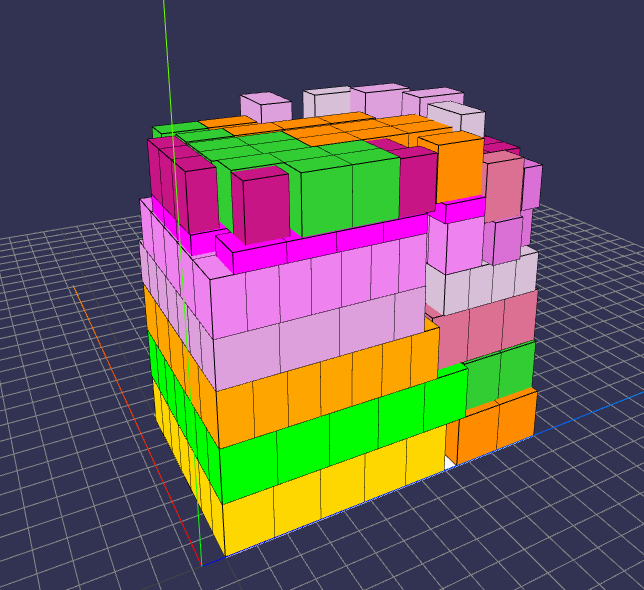
\includegraphics[width = 3in]{tests/usecase/instance-95_k200.PNG}} 
    \subfloat[Instance 82]{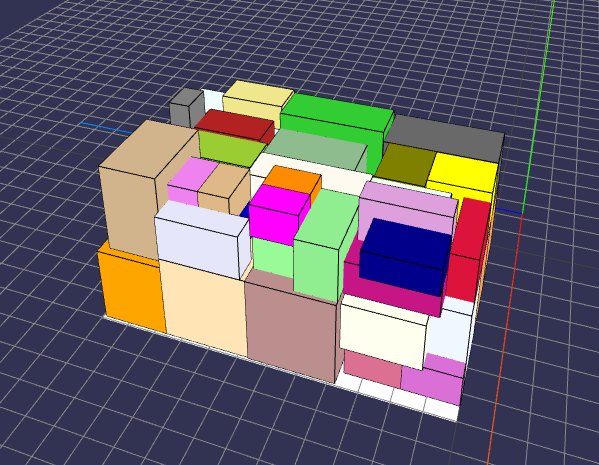
\includegraphics[width = 3in]{tests/usecase/instance-82_k200.PNG}}\\
    \subfloat[Instance 56]{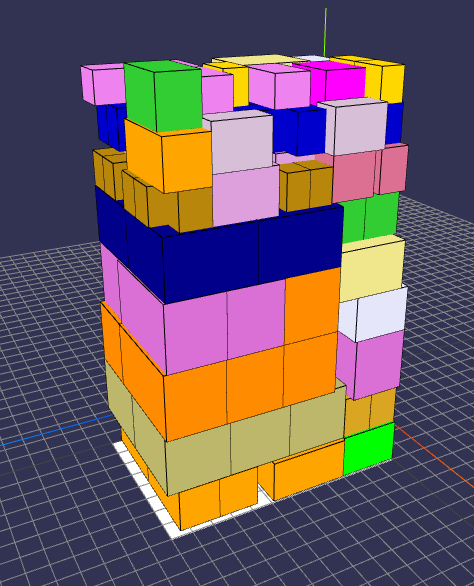
\includegraphics[width = 3in]{tests/usecase/instance-56_k200.PNG}} 
    \subfloat[Instance 66, Bin 1]{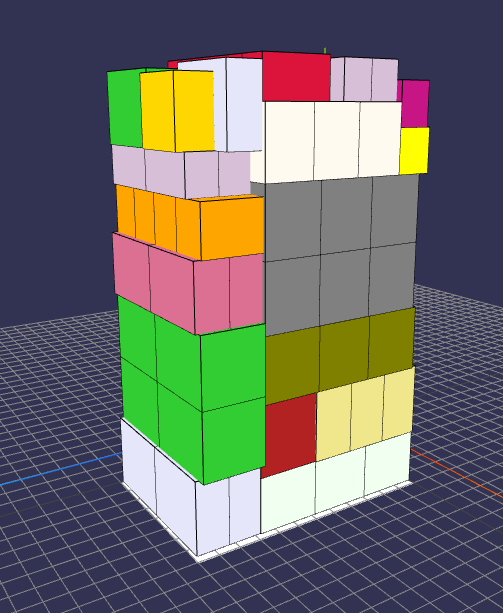
\includegraphics[width = 3in]{tests/usecase/instance-66_bin1_k200.PNG}}
    \caption{Some solutions of the use-case tests with the "Group by Hash" behaviour and $k=200$}
    \label{fig:usecase_tests}
\end{figure}

    \chapter{Conclusions and future developments}
    \label{chapther:conclusions}%
    A final chapter containing the main conclusions of your research/study
and possible future developments of your work have to be inserted in this chapter.
    %FIXME: Remove
    \cite{knuth74} 

    %-------------------------------------------------------------------------
    %	BIBLIOGRAPHY
    %-------------------------------------------------------------------------

    \addtocontents{toc}{\vspace{2em}} % Add a gap in the Contents, for aesthetics
    \bibliography{literature} % The references information are stored in the file named "literature.bib"

    %-------------------------------------------------------------------------
    %	APPENDICES
    %-------------------------------------------------------------------------

    \cleardoublepage
    \addtocontents{toc}{\vspace{2em}} % Add a gap in the Contents, for aesthetics
    \appendix
    \chapter{Appendix A}
    If you need to include an appendix to support the research in your thesis, you can place it at the end of the manuscript.
    An appendix contains supplementary material (figures, tables, data, codes, mathematical proofs, surveys, \dots)
    which supplement the main results contained in the previous chapters.

    \chapter{Appendix B}
    It may be necessary to include another appendix to better organize the presentation of supplementary material.


    % LIST OF FIGURES
    \listoffigures

    % LIST OF TABLES
    \listoftables

    % LIST OF SYMBOLS
    % Write out the List of Symbols in this page
    \chapter*{List of Symbols} % You have to include a chapter for your list of symbols (
    \begin{table}[H]
        \centering
        \begin{tabular}{lll}
            \textbf{Variable} & \textbf{Description} & \textbf{SI unit} \\\hline\\[-9px]
            $\bm{u}$ & solid displacement & m \\[2px]
            $\bm{u}_f$ & fluid displacement & m \\[2px]
        \end{tabular}
    \end{table}

    % ACKNOWLEDGEMENTS
    \chapter*{Acknowledgements}
    Here you might want to acknowledge someone.

    \cleardoublepage

\end{document}